\documentclass{Quintorthesis} 

\usepackage[utf8]{inputenc}
\usepackage{colortbl}
\usepackage[export]{adjustbox}
\usepackage{booktabs}
\usepackage{graphicx, hyperref, parskip, subcaption, float, fancyhdr, amsmath, mathtools, wrapfig, color, titlesec }
\usepackage[dutch]{babel}
\usepackage{listings}
\usepackage{enumitem}
\usepackage[font={small, it}]{caption}
\usepackage[toc,page]{appendix}
\usepackage[natbibapa]{apacite}
\usepackage{pdfpages}
\usepackage[acronym]{glossaries}
\usepackage{glossary-mcols}
\usepackage{bookmark}

\newcommand{\source}[1]{\caption*{Source: {#1}} }
\newcommand{\R}{\mathbb{R}}
\newcommand*{\Scale}[2][4]{\scalebox{#1}{$#2$}}%

\setglossarystyle{mcolindexgroup}
\makenoidxglossaries
\loadglsentries{begrippen}

\begin{document}
  \baselineskip=15pt plus1pt
  \parskip=15pt
  \setcounter{secnumdepth}{2}
  \setcounter{tocdepth}{3}

  \renewcommand\appendixpagename{Bijlages}
  \renewcommand\appendixtocname{Bijlages}
  \newcommand{\hsp}{\hspace{10pt}}

  % Custom spacings for chapter, paragraph and textcolors
  \titleformat{\chapter}[hang]{\Huge\bfseries}{\thechapter\hsp\textcolor{quintorred}{|}\hsp}{0pt}{\LARGE\bfseries}
  \titlespacing*{\chapter}{0pt}{0pt}{20pt}
  \titlespacing*{\paragraph}{0pt}{0pt}{10pt}

  \begin{titlepage}
    \documenttype{Onderzoek naar} 
    \title{Gedistribueerde netwerken en identiteits management binnen Blockchain technologie}
    \author{Jeffrey van Hoven}
    \date{\today}
    \maketitle
  \end{titlepage}

  % Start of Roman Pages. Here goes the preface, definitions 
  % and abstract
  \begin{romanpages}
    \chapter*{Voorwoord}

Voor u ligt mijn afstudeerverslag; ``\textit{Het realiseren van een gedistribueerd netwerk met mogelijkheid tot identiteit management ter behoeve van Blockchain technologie}'' waarin ik schrijf over de uitvoering van het onderzoek dat gedaan is ten behoeve van mijn afstuderen voor de opleiding Informatica aan de Haagse Hogeschool. Het betreft verslaglegging van het proces dat doorlopen is om de uitdagende opdracht zoals voorgesteld door Quintor uit te voeren.

In de opdracht is er na uitvoerig onderzoek tot de conclusie gekomen welke technieken geschikt zijn om toegepast te kunnen worden om de Blockchain onderdelen Distributed Network en Identity Management te realiseren. Gedurende het afstudeertraject kon ik altijd met vragen terecht bij zowel mijn bedrijfsbegeleider, Ben Ooms, als de Blockchain expert, Pim Otte.

Hierbij bedank ik mijn begeleiders, vanuit Quintor en vanuit de opleiding, voor hun begeleiding, inzichten en ondersteuning tijdens het afstudeertraject. Daarnaast wil ik graag mijn mede afstudeerders bedanken voor hun meedenken en inzichten in het vinden van oplossingen. In het bijzonder bedank ik mede afstudeerder Kevin Bos, waarmee de samenwerking gedurende de opdracht aangenaam en productief is geweest. 

Als laatste bedank ik mijn familie en vrienden voor hun ondersteuning, indirect of direct, niet alleen tijdens het afstuderen, maar ook tijdens mijn studieloopbaan. Zonder hun ondersteuning zou dit mogelijk geweest zijn.

Ik wens u veel leesplezier toe.

\bigskip
\bigskip

Jeffrey van Hoven \\
Den Haag, 1 juni 2018

    \tableofcontents     
    \listoffigures              
    \listoftables
    \printnoidxglossary[title=Woordenlijst]
    \printnoidxglossary[title=Afkortingen, type=\acronymtype]
  \end{romanpages}

  \chapter{Inleiding}

Dit verslag is geschreven in het kader van mijn afstudeeropdracht bij Quintor en dient ter beoordeling van de werkzaamheden die uitgevoerd zijn voor de bachelorstudie Informatica aan de Haagse Hogeschool. 

Door de snelle groei van het Blockchain domein heeft Quintor in 2017 in samenwerking met DUO/MinOCW, Groningen Declaration Network, Stichting ePortfolio Support, TNO en Rabobank, het Blockchain Field-lab Education gestart in Groningen. Het Blockchain-lab is opgezet om expertise en kennis uit te wisselen op regionaal, nationaal en internationaal gebied. De oprichting van het Blockchain Field-lab Education heeft er mede voor gezorgd dat Quintor meer kennis wilt opdoen over het Blockchain domein om zo inzicht te krijgen in hoe Blockchain technologie ingezet kan worden binnen vraagstukken vanuit klanten. 

In hoofdstuk 2 is de organisatie beschreven waar het afstudeertraject heeft plaatsgevonden. Vervolgens wordt in hoofdstuk 3 de opdracht gepresenteerd. In hoofdstuk 4 wordt de aanpak van de opdracht onderbouwd en in hoofdstuk 5 wordt de orientatie van de opdracht besproken. In hoofdstuk 6 worden de werkzaamheden van het vooronderzoek besproken waarin de basis van Blockchain technologie ter sprake komt. In hoofdstuk 7 wordt het hoofdonderzoek naar de segmenten Identity Management en Distributed Network in bestaande Blockchain implementaties beschreven. Hoofdstuk 8 presenteert het advies dat gegeven wordt naar aanleiding van het gedane onderzoek. Hoofdstuk 9 beschrijft de totstandkoming van het ontwerp voor de architectuur. In hoofdstuk 10 worden de keuzes die gemaakt zijn voor de indeling van het Proof of Concept beschreven en wordt er kort uitgelicht hoe de realisatie van het Peer-to-Peer netwerk is verlopen. In hoofdstuk 11 wordt er geëvalueerd over de producten, de aanpak, de geselecteerde beroepstaken, het functioneren in het bedrijf en de leerpunten die getrokken zijn uit het project. Tot slot worden er in hoofdstuk 11 aanbevelingen gegeven voor vervolgonderzoek.

  \chapter{Quintor}
\textit{In dit hoofdstuk zal er inzicht gegeven worden over het bedrijf Quintor waar het afstudeerproject heeft plaatsgevonden. Er wordt verteld over de diensten die Quintor levert en wat de doelen zijn van de organisatie. Er zal ook kort toegelicht worden waar de afstudeerder binnen het bedrijf opereert en welke werknemers vanuit Quintor betrokken zijn bij de afstudeeropdracht.
}

Quintor is een toonaangevend bedrijf op het gebied van Agile software development, Enterprise Java / .NET technologie en mobile development. Het bedrijf is begonnen in 2005 in Groningen en is opgericht door Johan Tillema, de huidige CEO van het bedrijf. Sinds 2005 heeft het bedrijf een gezonde groei doorgemaakt en heeft inmiddels 150 medewerkers, verspreid over vestigingen in Groningen, Amersfoort en Den Haag. Vanuit deze vestigingen ondersteunt het bedrijf klanten bij de uitdagingen die grootschalige Enterprise projecten met zich meebrengen. Het succes van Quintor is te danken aan drie pijlers: techniek en architectuur, een hoogwaardige ontwikkelstraat en het Agile/Scrum proces. Tevens beschikt Quintor over een Software Factory waarin in-house projecten voor klanten worden uitgevoerd.

\section{Software Factory}

In de Software Factory staat alle kennis en expertise die Quintor heeft verzameld over de jaren heen. Het is een hoogwaardig platform waarin de tooling, standaarden en best practices en tevens een complete oplossing is voor het managen en hosten van Scrum projecten. Dit wordt onder andere gebruikt om klanten te helpen bij het professionaliseren en efficiënter inrichten van softwareontwikkeling. Een groot deel van de werkzaamheden die Quintor dan ook uitvoert voor klanten is consultatie bij o.a. het implementeren van Agile/Scrum werk- en denkwijze. Naast Java en .NET development behoort ook mobile development tot de kerncompetenties van Quintor, en is dan ook opgenomen in de Software Factory. Hieronder zijn een aantal onderdelen uitgelicht die voorkomen in de Software Factory.

\paragraph{Enterprise architectuur}

Vanuit een pragmatische insteek en op basis van jarenlange ervaring helpen de software architecten van Quintor organisaties bij het maken van de juiste keuzes op het gebied van architectuur. Hierbij gaat het om het zowel opstellen als implementeren van een architectuur.

\paragraph{Informatie analyse}

Het in kaart brengen van informatie door het gebruik van diverse analyse- en ontwerptechnieken zoals UML, user-stories en use-cases in een Agile omgeving.

\paragraph{Java en .NET development}

Het realiseren van duurzame IT-systemen, in-house of bij klanten, die naadloos aansluiten bij de wensen van de business. Hierbij zijn er een groot aantal van omvangrijke systemen ontwikkelt.

\paragraph{Agile/Scrum}

Agile/Scrum is een effectieve en flexibele methode die uitgaat van een iteratiefontwikkelproces. Het trainen van complete projectteams met een op maat gemaakte training, waarbij aansluitend support en coaching gegeven wordt.

\paragraph{Mobile development}

Mobiele applicaties voor iPhone, iPad en Android. Specifiek hiervoor is het 'Mobile development center' opgezet, waarin er apps ontworpen, ontwikkelt en beheert worden. Dit betreft de realisatie van stand-alone tot volledige geïntegreerde Enterprise apps.

\section{Visie}

Een van de doelstellingen die Quintor heeft is het professionaliseren van software development. Aansluitend daarop probeert het bedrijf continu voor te lopen op de concurrentie door het opdoen van kennis op het gebied van nieuwe technologieën, waarbij professionalisering van de werkwijze voorop staat.

\begin{formal}
  \label{visie}
  ``Onze ambitie: professionaliseren van software development."
  \\ Johan Tillema, Chief Executive Officer
\end{formal}

Door het aanbieden van uitdagende afstudeeropdrachten wordt er kennis opgebouwd die benodigd is om nieuwe technologieën, zoals bijvoorbeeld Machine Learning of Blockchain, in te zetten om klanten te adviseren bij de uitdagingen die grootschalige Enterprise projecten met zich meebrengen en zal, middels het volwassen genoeg is, opgenomen worden in de Software Factory.

\section{Organisatie}
In fig. \ref{organogram} wordt de organisatie van Quintor weergegeven. Bovenaan staat Johan Tillema, de oprichter en CEO. Direct eronder staat het Secretariaat en het Recruitment Office. Hierin is te zien dat er vier segmenten zijn waarop er consultatie aangeboden wordt: development, analysis en design en front-end.

\begin{figure}[h]
  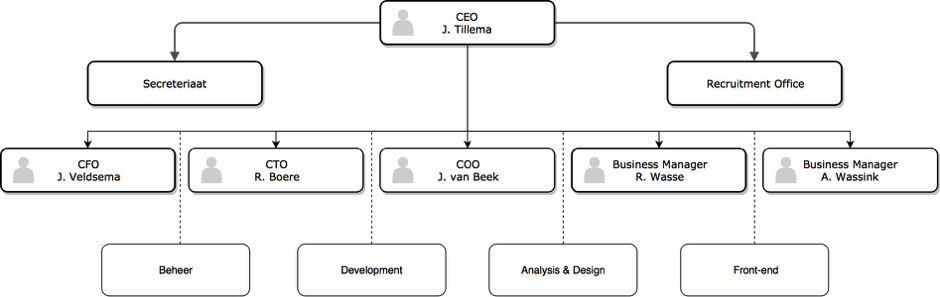
\includegraphics[width=1\textwidth]{figures/organogram}
  \caption{Organogram van Quintor.}
  \label{organogram}
\end{figure}

\newpage
Zelf val ik onder het development segment, waarbij er aangestuurd wordt door Ben Ooms, (beschreven in \ref{begeleider}). Er wordt zelfstandig gewerkt aan de opdracht waarbij er een aantal praktijken van Scrum toegepast zijn tijdens het afstudeertraject. Zo is er elke twee weken een zogenaamde demo dag waarbij iedere afstudeerder een demonstratie over waar hij of zij de afgelopen tijd mee bezig is geweest, en of er ergens tegenaan gelopen wordt zodat er samen nagedacht kan worden over mogelijke oplossingen.

\section{Infrastructuur}

Quintor maakt intensief gebruik van het Agile principe en dit is dan ook terug te vinden in de infrastructuur die ingericht is voor de consultanten binnen Quintor. Voor het uitvoeren van projecten wordt Atlassian JIRA gebruikt om het Agile proces te ondesteunen. Hierin is het mogelijk om taken te creëren en toe te wijzen aan projecten. Elke taak is dan individueel op te pakken door een team die op een bepaald project gezet is. 

Voor het waarborgen van de kwaliteit van de software wordt er gebruik gemaakt van Atlassian BitBucket. BitBucket is een web-based versiebeheer systeem dat het Mercurial of Git revisiesystemen ondersteund. Daarnaast werkt het uitstekend samen met JIRA, waarbij het mogelijk is om naar taken die opgepakt zijn binnen JIRA te refereren binnen BitBucket.

Communicatie binnen de organisatie gaat via het interne mail-systeem die functionaliteiten ondersteund zoals bijvoorbeeld het interne chat-systeem waarbij het mogelijk is om elke medewerker te benaderen en een kalender die het mogelijk maakt om afspraken te koppelen aan medewerkers en locaties.

\section{Betrokkenen}

Binnen Quintor zijn er een aantal medewerkers die nodig zijn om het project tot een geslaagd einde te brengen. Hieronder zijn deze medewerkers kort benoemd en wat hun rol is binnen het afstudeertraject.

\paragraph{Ben Ooms} \label{begeleider} is de teamleider van Quintor Den Haag en is tevens de begeleider tijdens het afstudeertraject. Zijn uitvoerende taken hierbij zijn dan ook onder andere advies geven over de aanpak van de opdracht en waarbij mogelijk de voortgang van de opdracht te waarborgen.

\paragraph{Pim Otte} \label{expert} is de Blockchain expert binnen Quintor en heeft veelal ervaring met de toepassing en realisatie van applicaties die gebruik maken van Blockchain technologie. Hij is beschikbaar gedurende de afstudeeropdracht om inzichten en feedback te geven op de uitgevoerde werkzaamheden.

\paragraph{Kevin Bos} is afstudeerder afkomstig van Avans Hogeschool. Hij is verantwoordelijk voor het lokale gedeelte van de Blockchain opdracht. Tijdens de afstudeeropdracht is hij een stakeholder van het project en zal er een zekere mate van samenwerking aanwezig zijn.
  \chapter{Opdracht}

In 2017 heeft Quintor in samenwerking met DUO/MinOCW, Groningen Declaration Network, Stichting ePortfolio Support, TNO en Rabobank, het Blockchain Field-lab Education gestart in Groningen. Het Blockchain-lab is opgezet om expertise en kennis uit te wisselen op regionaal, nationaal en internationaal gebied. De oprichting van het Blockchain Field-lab Education heeft er mede voor gezorgd dat Quintor meer kennis wilt opdoen op het gebied van Blockchain. Daarnaast bestaat er de mogelijkheid dat het bedrijf in de toekomst Blockchain technologie wilt inzetten om vraagstukken vanuit klanten op te lossen.

\begin{figure}[h]
  \centering
  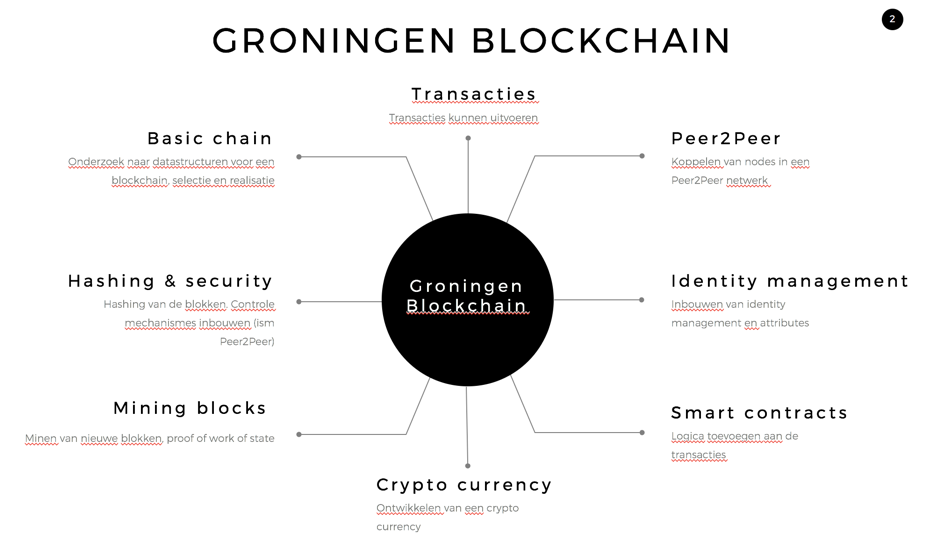
\includegraphics{figures/indeling_blockchain_opdracht}
  \caption{Indeling opdracht Blockchain ontwikkeling zoals gegeven door Quintor afkomstig uit.}
  \label{indeling_blockchain_opdracht} 
\end{figure}

De focus in de afstudeeropdracht ligt op de Blockchain onderdelen Identity Management en Peer2Peer (Distributed Network). Dit zal in samenwerking gaan met een andere afstudeerder, Kevin Bos, die verantwoordelijk is voor de onderdelen Basic chain, Hashing \& security en Mining blocks. 

\newpage
\section{Probleemstelling}

Sinds de opkomst van Bitcoin is de Blockchain technologie, de techniek die het mogelijk maakt om het op een gedecentraliseerde manier te laten werken, steeds populairder geworden. Alhoewel de Blockchain-technologie nog in de kinderschoenen staat, gaan de ontwikkelingen in het domein zeer snel. Zo worden er toepassingen bedacht die niet alleen voor de financiële markten interessant zijn, maar ook voor bijvoorbeeld het digitaliseren van contracten en contractbeheer.

Aangezien de toepassing en adoptie van Blockchain technologie steeds groter wordt wil Quintor de toepassingsmogelijkheden en technieken onderzoeken om zo inzicht te kunnen krijgen in hoe het gebruikt kan worden in de aangeboden vraagstukken vanuit klanten.

\section{Doelstelling}

De doelstelling van de opdracht is verspreid over onderdelen van Blockchain technologie, zoals te zien in fig. \ref{indeling_blockchain_opdracht}. Hierdoor is er een globaal doel en een doel die specifiek voor deze opdracht geldt. Het streven naar het globale doel is het opdoen van kennis omtrent het realiseren van een Blockchain implementatie. Het doel van deze specifieke opdracht is middels het opstellen van een proof-of-concept van de Blockchain onderdelen Identity Management en Distributed Network, zonder gebruik te maken van bestaande Blockchain protocollen, kennis te ontwikkelen voor Quintor op het gebied van Blockchain technologie.

\section{Resultaat}

Indien de opdracht succesvol afgerond is, zijn de onderdelen Identity Management en het Peer2Peer netwerk gerealiseerd aan de hand van voorgestelde technieken die voortgekomen zijn uit het gedane onderzoek. In samenwerking met de onderdelen die gerealiseerd zijn door Kevin Bos zal er een werkend Proof of Concept van een Blockchain gerealiseerd zijn. Zowel het Proof of Concept als het onderzoek zal voor Quintor inzicht bieden in het Blockchain domein en de ontwikkelingen daarin.

\subsection{Producten}

Als onderdeel van de afstudeeropdracht zullen er verschillende producten worden opgeleverd aan Quintor en aan de Haagse Hogeschool. Deze staan hieronder gespecificeerd.

De op te leveren producten aan Quintor zijn:
\begin{itemize}
  \item{Adviesrapport}
  \item{Sprint demo presentaties}
  \item{Broncode van de ontwikkelde applicatie}
  \item{Opgestelde documentatie}
\end{itemize}

De op te leveren producten aan de Haagse Hogeschool zijn:
\begin{itemize}
  \item{Afstudeerscriptie}
  \item{Plan van Aanpak}
  \item{Adviesrapport}
  \item{Testrapport}
  \item{Technisch ontwerp}
\end{itemize}



  \chapter{Aanpak}
\label{Aanpak}

\textit{In dit hoofdstuk wordt de totstandkoming van de aanpak voor de opdracht besproken. Het gaat uit van de beginsituatie zoals beschreven in het afstudeerplan, in te zien in bijlage \ref{appendix:afstudeerplan}. Daarnaast worden de afwijkingen besproken tegenover de originele opdracht, zoals geformuleerd in hoofstuk 3.}

\section{Inrichting}

Aangezien Quintor een groot voorstander is van het Agile werken zien zij ook graag het afstudeertraject in die vorm uitgevoerd worden. Tijdens de studie is er veel ervaring opgedaan met het Scrum framework dat het Agile principe ondersteund waardoor het een logische keuze is om de structuur van het project te bepalen. Omdat een groot gedeelte van het project bestaat uit het individueel uitvoeren van onderzoek zijn niet alle best practices overgenomen. 

De rollen binnen het scrum proces \citep{schwaber2011scrum} zijn als volgt gedefinieerd:
\begin{itemize}[noitemsep]
  \item \textbf{Scrum Master} - Ben Ooms
  \item \textbf{Product Owner} - Johan Tillema / Ben Ooms
  \item \textbf{Development Team} - Jeffrey van Hoven
\end{itemize}

Een sprint zal bestaan uit twee weken waarbij aan het eind van de sprint een demo van de huidige status van het project wordt gegeven aan de afstudeerbegeleider vanuit Quintor. Tijdens dit moment is het mogelijk om advies te krijgen over de uitvoering van de werkzaamheden of blokkades waar tegenaan gelopen wordt. Daarnaast wordt er onder de afstudeerders dagelijks een stand-up gehouden waarin zaken zoals de status van het project, welke werkzaamheden gepland staan voor de dag en of er obstakels zijn besproken worden.
\subsection{Fases}

Er wordt uitgegaan van drie fases binnen het project: \textbf{onderzoek}, \textbf{ontwerp} en \textbf{realisatie}, waarbij de fases ontwerp en realisatie Agile uitgevoerd worden volgens de Scrum richtlijnen.

\newpage
\section{Fase 1: Onderzoek}
\subsection{Vooronderzoek}

In het afstudeertraject wordt er met technologieën gewerkt welke onbekend zijn. Er is er dan ook voor gekozen om aan de hand van vooronderzoek kennis op te doen over het Blockchain domein. Er zal eerst onderzocht worden wat een Blockchain is waarna er ingegaan wordt op de toepassing van de techniek. Vervolgens zal er worden gekeken naar de architectuur van de Blockchain en uit welke componenten het bestaat. Uiteindelijk zal er kennis opgedaan worden voor de onderdelen Identity Management en Distributed Network om zo een afbakening te creëren van de onderdelen. Deze kennis zal gebruikt worden, in overleg met Quintor, om de opdracht vorm te geven en inzichten op te doen over de mogelijkheden met de opdracht.

\subsubsection{Dataverzameling}
Voor het opdoen van voorkennis zullen er gepubliceerde research papers, wiki’s en blogs gebruikt worden. Hierna zal er een selectie van Blockchain implementaties gemaakt worden die bestudeerd zullen worden in het onderzoek.
\subsection{Hoofdonderzoek}

Voor het uitvoeren van het onderzoek zal ik gebruik maken van deskresearch. Voor mijn deskresearch zullen er specifieke cases van Blockchain implementaties geanalyseerd worden op de segmenten Distributed Network en Identity Management. Hiervoor zal ik proberen een zo compleet mogelijk technische beschrijving van de werking van deze segmenten op te stellen.

In de opdrachtomschrijving die aangeleverd is door Quintor zijn er geen duidelijke eisen en specificaties gesteld aan zowel de uitvoering als realisatie van de afstudeeropdracht. Dit heeft ertoe geleid dat er een gesprek gehouden is met de Blockchain expert en de bedrijfsbegeleider over de eisen, afbakening en in welke mate de samenwerking met de andere afstudeerder benodigd zal zijn. Hieruit is naar voren gekomen dat er wederom geen specifieke eisen zijn en dat de afstudeerder onderzoek dient te doen naar implementaties om een zo goed mogelijk functioneel overzicht te creëren van de onderdelen die toegekend zijn. Omdat de missie van Quintor het vooroplopen op het gebied van IT ontwikkelingen is, is ervoor gekozen om exploratief onderzoek uit te voeren.

\section{Fase 2: Ontwerpen}
Uit het hoofdonderzoek zullen methoden en technieken geselecteerd worden die gerealiseerd zullen worden in een Proof of Concept. Alvorens deze gerealiseerd zal worden moet er nagedacht worden over hoe dit eruit zal komen te zien op technisch gebied. Het modelleren, implementeren en documenteren van een systeem vereist dat het systeem vanuit verschillende aspecten wordt bekeken. Er zal een keuze gemaakt worden betreft een methode voor het faciliteren van deze filosofie.


\section{Fase 3: Realisatie}
\subsection{Ontwikkeling}

De uitgekozen technieken zullen gerealiseerd worden in een Proof of Concept. Dit zal in samenwerking zijn met de andere afstudeerder, die het lokale gedeelte van de Blockchain ontwikkeld. De onderdelen dienen samen te werken tot een functionele Blockchain implementatie, waarbij er overlap zal zijn in de keuzes binnen de pakketselectie en realisatie.

\paragraph{Requirements} Er dienen criteria opgesteld te worden aan de hand van het resultaat van het onderzoek die van toepassing zijn op de realisatie van het Proof of Concept. Om te achterhalen wat de eisen en de toepassing waaraan het Proof of Concept moet voldoen zullen er informele interviews gehouden worden waarin requirements achterhaald worden.

\paragraph{Selecteren methoden} Voor het opzetten van een development workflow en de technieken die daarbij te pas komen in overeenstemming met Quintor zullen er beslissingen gemaakt worden op de manier waarop het Proof of Concept gerealiseerd gaat worden. Tevens zal hierbij gekeken worden naar de uitvoering van realisatie op bestaande implementaties.


% \subsection{Adviesrapport}
% TODO: Wat moet hiermee gebeuren?
% Om in overeenstemming met de opdrachtgever een toepassing te kiezen voor de functionaliteiten en/of technieken die onderzocht zijn in de geselecteerde protocollen, zal er een adviesrapport opgesteld worden waarin deze technieken en/of technologieën aangeraden worden. 

\clearpage
\section{Planning}
Er is een globale planning gemaakt die uitgaat van de drie gestelde fases: \textbf{onderzoek}, \textbf{ontwerp} en \textbf{realisatie}. Er wordt ervan uitgegaan dat elk van deze fases ongeveer \( \frac{1}{3} \)de van de tijd in beslag zal nemen. Aangezien de fases ontwerp en realisatie Agile uitgevoerd worden wordt er vanuit gegaan dat er niet veel tijd besteed zal worden aan het ontwerpen alvorens begonnen wordt aan de realisatie. Binnen deze drie fases zal er tijd gealloceerd worden voor het inventariseren, opzetten en opdoen van benodigde kennis en documentatie. In onderstaand tabel is een globale planning opgezet voor de drie fases.

\begin{table}[ht]
  \begin{tabular}{|p{6cm}|p{4cm}|p{4cm}|}
    \hline
    \textbf{Fase} & \textbf{Van} & \textbf{Tot en met} \\
    \hline
    Onderzoek & Week 3 & Week 9 \\
    \hline
    Ontwerp & Week 10 & Week 17 \\
    \hline
    Realisatie & Week 11 & Week 17 \\
    \hline
    Afronding & Week 18 & - \\
    \hline
  \end{tabular}
  \caption{Globale planning}
  \label{planning}
\end{table}

Waarbij de werkzaamheden die uitgevoerd zullen worden binnen een fase er ongeveer als volgt uitzien:

\begin{multicols}{2}
  \begin{itemize}[noitemsep]
    \item \textbf{Onderzoek}
    \begin{itemize}[noitemsep]
      \item Vooronderzoek
      \item Selectie implementaties
      \item Onderzoeksopzet
      \item Onderzoek
      \item Advies
    \end{itemize}
    \item \textbf{Ontwerp}
    \begin{itemize}[noitemsep]
      \item Selecteren methode
      \item Ontwerp individuele views
    \end{itemize}
    \item \textbf{Realisatie}
    \begin{itemize}[noitemsep]
      \item Informatieplan
      \item Realisatie in vorm van sprints
      \item Testen
    \end{itemize}
    \item \textbf{Afronding}
    \begin{itemize}
      \item Overdracht
      \item Afronding afstudeerverslag
    \end{itemize}
  \end{itemize}
\end{multicols}
  \chapter{Vooronderzoek en resultaten}

\textit{In dit hoofdstuk wordt er een introductie gegeven in het Blockchain domein. Deze kennis is benodigd om het onderzoek uit te voeren en om het Proof of Concept te realiseren. Daarnaast zal deze kennis helpen om de uitvoering van de opdracht te begrijpen. Het vooronderzoek dient tevens om overeenstemming te krijgen met de opdrachtgever over de richting van het onderzoek. Zoals verteld in de aanpak zijn er weinig eisen gesteld aan de uitvoering en toepassing van de afstudeeropdracht, waardoor het wenselijk is om een gezamenlijke overeenstemming te krijgen van wat mogelijk is met het onderzoek.}

Het vooronderzoek betreft kwalitatief-, exploratief onderzoek dat uitgevoerd wordt door middel van deskresearch. De reden dat ik hiervoor heb gekozen is omdat het Blockchain domein nieuw voor mij is en ik dus ook niet welke specifieke kennis ik nodig heb om de vragen te beantwoorden. De bronnen die ik gebruikt heb zijn zowel informeel als formeel waarbij er veel informatie afkomstig is uit het Bitcoin protocol, zoals beschreven door \cite{nakamoto2008bitcoin}. Dit is een van de meest gedocumenteerde Blockchain implementaties die publiekelijk in te zien is. Om de technische kennis te versterken voor de realisatie van het Proof of Concept is er een Coursera course gevolgd, Bitcoin and Cryptocurrency Technologies, waarin het Bitcoin protocol uitgelegd wordt. Dit is gevolgd omdat de beschrijving van het Bitcoin protocol niet meer toereikend is naar de huidige staat van de implementatie.

Er wordt ingegaan op de basis van Blockchain technologie waarna er gekeken wordt naar de mogelijke toepassingen. Vervolgens komt de architectuur van een Blockchain aan bod, waarbij de vraag ``Uit welke componenten bestaat een Blockchain implementatie?" wordt behandeld. Om een afbakening te maken voor het onderzoek wordt er gekeken naar wat de onderdelen Distributed Network en Identity Management bevatten. Concreet staan de vragen die behandeld worden in het vooronderzoek hieronder weergegeven.

\begin{enumerate}[noitemsep]
  \item Wat is Blockchain technologie?
  \item Waarvoor wordt Blockchain technologie gebruikt?
  \item Uit welke onderdelen bestaat een Blockchain?
  \item Waaruit bestaat het onderdeel Distributed Network binnen Blockchain technologie?
  \item Waaruit bestaat het onderdeel Identity Management binnen Blockchain technologie?
\end{enumerate}

\newpage
\section{Blockchain}
\label{chapter:blockchain}

\textit{
  In dit hoofdstuk wordt de vraag  ``Wat is Blockchain technologie?" behandeld. Het betreft het vergaren van kennis over de basis van het Blockchain begrip waarbij er ingegaan wordt op wat Blockchain is en welke eigenschappen het heeft. Door het beantwoorden van deze vraag wordt er een definitie vastgesteld van Blockchain technologie die gebruikt wordt in het gehele verslag.
}

Een blockchain is een gedistribueerde database die bestaat uit een keten van in de computer of op internet vastgelegde en samengevoegde gegevens genaamd blocks. Om deze reden wordt blockchain technologie ook wel vergeleken met een grootboek. In zekere mate is dit correct maar het omschrijft niet het meest vooraanstaande aspect van blockchain, namelijk dat het gedecentraliseerd opereert.

Om de analogie voort te zetten; een grootboek is in handen van één organisatie waarin transacties van of naar de organisatie vastgelegd worden. Dit betekent dat er een centrale autoriteit is die kan bepalen of er überhaupt wel transacties plaatsvinden, of erger, het systeem buiten gebruik kan stellen. Daarnaast is de centrale autoriteit ook in staat misbruik te maken door bijvoorbeeld transacties te registreren naar de eigenaar van het grootboek. Dit brengt een risico met zich mee die blockchain technologie oplost door het grootboek te verspreiden over een netwerk dat ervoor zorgt dat deze centrale autoriteit niet meer nodig is.

Een traditionele blockchain is weergegeven in fig. \ref{blockchain_reference}. De keten van gegevens wordt bepaald door de volgorde waarin de gegevens zijn toegevoegd. Er is daarbij een eenvoudig te controleren systeem volgens welke voorafgaande blokken aan elkaar gerelateerd behoren te zijn. Door de inhoud van het vorige block crypto grafisch te versleutelen (ook wel hashen genoemd) en deze sleutel op te nemen in een opeenvolgend blok wordt ervoor gezorgd dat gegevens van eerdere blokken niet meer gemuteerd kunnen worden. Wanneer dit wel gebeurt zou de ketting verbroken worden omdat er een nieuwe sleutel gegenereerd wordt en opeenvolgende blokken zullen refereren naar een foutieve sleutel.
  
\begin{figure}[h]
  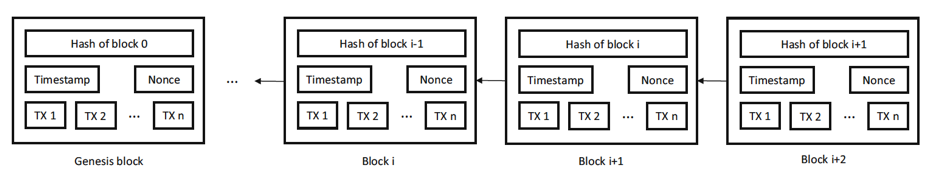
\includegraphics[width=1\textwidth]{figures/blockchain}
  \caption{Voorbeeld van een blockchain \citep{zheng2016blockchain}}
  \label{blockchain_reference}
\end{figure}

\clearpage
\subsection{Eigenschappen}

\cite{zheng2017overview}[Key Characteristics of Blockchain, p.5] stelt dat er vier eigenschappen zijn die een Blockchain definiëren:

\paragraph{Decentralisatie} In traditionele gecentraliseerde transactie systemen wordt iedere transactie gevalideerd door een centrale vertrouwde organisatie (e.g.\ banken), waardoor er een bottleneck gecreëerd wordt door de transacties te verwerken door centrale informatiesystemen. In contrast daarmee is een derde partij niet meer nodig in blockchain systemen. Consensus algoritmes zorgen ervoor dat data consistent is binnen het netwerk.

\paragraph{Persisentie} Transacties kunnen snel gevalideerd worden en invalide transacties zullen niet toegelaten worden. Het is bijna onmogelijk om te transacties verwijderen of ongedaan te maken als ze zijn opgenomen in de blockchain.

\paragraph{Anonimiteit} Elke gebruiker van het systeem kan interacteren zonder zijn ``echte" identiteit kenbaar te maken.

\paragraph{Controleerbaarheid} In bitcoin wordt de balans van een gebruiker opgeslagen door gebruik te maken van het Unspent Transaction Output (UTXO) model. Elke transactie refereert naar eerdere unspent transacties. Wanneer de huidige transactie is opgenomen in de blockchain, zal de staat van alle gerefereerde transacties verandert worden van ``unspent" naar ``spent". Hierdoor zijn transacties makkelijk te valideren en te traceren.

\newpage
\section{Toepassing}

\textit{In dit hoofdstuk wordt de vraag ``Waarvoor wordt Blockchain technologie gebruikt?'' beantwoord. Deze vraag is opgesteld omdat er geen toepassing bekend is voor de te realiseren Blockchain onderdelen, zoals aangegeven in de beschrijving van de aanpak. Het antwoord op deze vraag dient om de opdrachtgever te informeren in wat er mogelijk is met Blockchain technologie om zo een toepassing te kiezen voor het te ontwikkelen Proof of Concept. \\ \\ Er is in het bijzonder aandacht geschonken aan Blockchain als development platform aangezien de opdrachtomschrijving, bijlage \ref{appendix:opdrachtformulering}, spreekt over de realisatie van het onderdeel Smart Contract. Uitleg over het onderdeel \glspl{smart_contract} is beperkt gebleven aangezien het buiten de scope van de opdracht valt.
}

Blockchain technologie wordt steeds vaker toegepast voor het opzetten van een gedecentraliseerd systeem. Aangezien de bekendste toepassing van blockchain technologie een financieel systeem is wordt het vaak gezien als technologie die specifiek bedoeld is om financiële diensten te ondersteunen. In de literatuur wordt er echter veel geëxperimenteerd en gespeculeerd over andere mogelijke toepassingen van blockchain technologie.

\begin{wrapfigure}{r}{0.5\textwidth}
  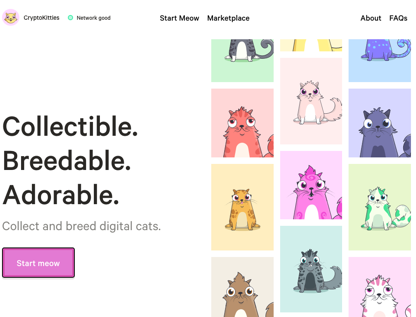
\includegraphics{figures/cryptokitties}
  \caption{CryptoKitties, een spel dat gebruik maakt van Blockchain technologie.}
  \label{cryptokitties}
\end{wrapfigure}

Zo stelt \citeauthor{atzori2015blockchain}, (\citeyear{atzori2015blockchain}) bijvoorbeeld dat blockchain technologie ingezet kan worden om de politiek en de maatschappij te veranderen. In een andere studie gedaan door \citeauthor{crosby2016blockchain}, (\citeyear{crosby2016blockchain}) wordt er onderscheid gemaakt tussen financiële en niet-financiële toepassingen die mogelijk veranderd kunnen worden door blockchain technologie. Een aantal voorbeelden die gegeven worden zijn de toepassingen bij verzekeringen, gedecentraliseerde opslag en domeinregistratie. In fig. \ref{cryptokitties} is een afbeelding te zien van de website van CryptoKitties, een van de eerste spellen die gebruik maakt van blockchain technologie, namelijk het Ethereum netwerk.

\clearpage
\subsection{Ontwikkelplatform}
Blockchains als Ethereum, EOS en HyperLedger bieden hun functionaliteit aan als development platform. Het stelt ontwikkelaars in staat om hun eigen toepassingen te realiseren, zogenaamde \gls{dapps}.

\begin{lstlisting}[
  linewidth=\textwidth, breaklines=true, 
  basicstyle=\small, label={smart_contract},
  caption={Smart contract voor ``The Greeter'' geschreven in Solidity, zoals gepresenteerd in een tutorial voor Smart Contracts op het Ethereum netwerk \citep{ethereum_smart_contract}.}]
  contract Mortal {
    /* Define variable owner of the type address */
    address owner;

    /* This function is executed at initialization and sets the owner of the contract */
    function Mortal() { owner = msg.sender; }

    /* Function to recover the funds on the contract */
    function kill() { if (msg.sender == owner) selfdestruct(owner); }
  }

  contract Greeter is Mortal {
    /* Define variable greeting of the type string */
    string greeting;

    /* This runs when the contract is executed */
    function Greeter(string _greeting) public {
        greeting = _greeting;
    }

    /* Main function */
    function greet() constant returns (string) {
        return greeting;
    }
  }
\end{lstlisting}

Door het gebruik van \glspl{smart_contract}, te zien in fig. \ref{smart_contract}, is het mogelijk om functionaliteit bij transacties te voegen om extra handelingen, die niet gerelateerd zijn tot de kern van een Blockchain implementatie, uit te voeren. Hieronder is een voorbeeld gegeven wat er mogelijk is met betrekking tot \gls{dapps}.

\paragraph{CryptoKitties} is een spel dat gebruikt maakt van het Ethereum platform, bestaand uit verzamelbare en fokbare digitale katten. De uitwisseling en het fokken van CryptoKitties wordt vastgelegd in het Ethereum netwerk door middel van \glspl{smart_contract}. Wanneer twee CryptoKitties gefokt worden, wordt het uiterlijk en de eigenschappen van hun nageslacht bepaald door het 256-bits genoom van elke ouder en een toeval element, wat leidt tot 4 miljard mogelijke genetische variaties \citep{cryptokitties}.


\newpage
\section{Architectuur}
\label{chapter:architecture}

\textit{
  In dit hoofdstuk wordt de vraag ``Uit welke componenten bestaat een Blockchain implementatie?'' behandeld. Het antwoord op deze vraag dient om een duidelijk beeld te scheppen welke componenten betrekking hebben op de onderdelen Distributed Network en Identity Management en tevens gebruikt zal worden als afstemming met zowel de opdrachtgever als de medeafstudeerder, Kevin Bos. 
}

\begin{wrapfigure}{r}{0.5\textwidth}
  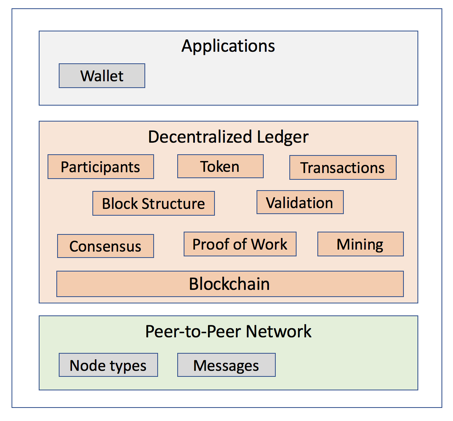
\includegraphics{figures/blockchain_architecture}
  \caption{Blockchain architectuur.}
  \label{blockchain_architecture}
\end{wrapfigure}

In fig. \ref{blockchain_architecture} is een overzicht weergegeven van de onderdelen en componenten waaruit een Blockchain bestaat. In de applicatie laag is de wallet te vinden die een gebruiker van de Blockchain doorgaans gebruikt om transacties te verrichten. De onderliggende functionaliteit van de wallet doet niets meer als het bijhouden van public- en private keys van de gebruiker waarop de nog niet uitgegeven tokens (cryptocurrency, contracten, diensten) geregistreerd staan.

De Decentralized Ledger is de kern van de technologie en zorgt ervoor dat de globale blockchain consistent en fraudebestending blijft. De fundamentele structuur achter de gehele technologie is de blockchain, waar transacties gegroepeerd worden in blokken en elk blok crypto grafisch verbonden wordt met het vorige blok. Een transactie is een vorm van uitwisseling van tokens tussen deelnemers, ook wel nodes genoemd, van het systeem. Voordat transacties als valide worden beschouwd, ondergaan ze een validatie proces die uitgevoerd wordt door alle nodes in het systeem. Het proces van het groeperen van transacties in een blok dat toegevoegd wordt aan het einde van de blockchain wordt ook wel minen genoemd. Om er zeker van te zijn dat er overeenstemming is onder alle deelnemers over welke blockchain legitiem is, wordt er gebruik gemaakt van een Proof-of-Work algoritme tijdens het mining proces om te bepalen welke ketting de meeste inspanning vereist.

Het laatste component is het peer-to-peer netwerk, waarin verschillende node types gedefinieerd zijn. Zo heb je bijvoorbeeld de validatie node die transacties valideert en een mining node die het mining process uitvoert. Om de Decentralized Ledger bij te werken en te onderhouden communiceren de nodes met elkaar door middel van het versturen van berichten.

\newpage
\section{Gedistribueerd netwerk}

\textit{
  In dit hoofdstuk wordt de vraag ``Waaruit bestaat het onderdeel gedistribueerd netwerk binnen Blockchain technologie?'' behandeld. Bij deze vraag wordt er gekeken naar de geïdentificeerde onderdelen uit hoofdstuk \ref{chapter:architecture}. Er wordt een korte introductie gegeven in peer-to-peer netwerken en waarom het een belangrijk onderdeel is bij het realiseren van de eigenschappen, behandeld in hoofdstuk \ref{chapter:blockchain}, van een Blockchain implementatie. Het antwoord op deze vraag zal helpen bij het selecteren van zoektermen die gebruikt worden om inventarisatie te doen op de onderdelen die het Distributed Network omvat.
}

Het onderdeel Distributed Network bestaat uit het verspreiden, uitbreiden en het behalen van consensus over de staat van de Blockchain tussen de deelnemers aan het netwerk. Om dit te doen wordt er gebruik gemaakt van een \acrfull{P2P} implementatie waarbij het mogelijk is om een lokale versie van de ketting aan te bieden aan andere nodes binnen het \acrshort{P2P} netwerk, om zo de huidige chain up-to-date te houden met wijzigingen die gedaan zijn door de verschillende verbonden nodes. Dit leidt tot een complex probleem dat beschreven wordt als het Byzantine Generals Problem \citep{lamport1982byzantine}, wat beschrijft aan de hand van een abstract voorbeeld dat het essentieel is voor een betrouwbaar computersysteem om te kunnen gaan met fouten die optreden in een of meer van de componenten, waardoor het kan voorkomen dat er conflicterende informatie verstuurd wordt naar de andere componenten van het systeem.

\textbf{Peer-to-Peer}

De term \acrshort{P2P} betekend dat alle computers die deel uit maken van het netwerk, peers van elkaar zijn, gelijk aan elkaar zijn, er geen speciale "nodes" zijn en dat alle deelnemers in het netwerk de last delen van het leveren van netwerkdiensten \citep[~p.171]{Antonopoulos:2014:MBU:2695500}. Het is een techniek die cruciaal is voor Blockchain en de doelen die het probeert te behalen. \acrshort{P2P} systemen verdelen namelijk de kosten om data te delen – opslag voor bestanden en bandbreedte voor het versturen van de bestanden – over de deelnemers van het netwerk, waardoor applicaties kunnen schalen zonder krachtige, dure servers \citep{bawa2003peer}.

Een van de bekendste toepassingen van een peer-to-peer netwerk is het creëren van een gedecentralizeerd file-sharing protocol. Implementaties hiervan zijn BitTorrent, LimeWire en Gnutella. Om een bestand te distribueren wordt het opgesplitst in delen, waarbij er een hash gecreëerd wordt voor elk deel. Wanneer een andere deelnemer van het netwerk een deel ontvangt wordt er gekeken aan de hand van de hash of het onderdeel geen fouten bevat. Bestanden worden geregistreerd in het netwerk door het opnemen van de hashes in een zogenaamde \textit{tracker} die gebruik maakt van een \acrfull{DHT}. Een voorbeeld van een DHT is te zien in fig. \ref{DHT}.

\newpage
\begin{wrapfigure}{l}{0.6\textwidth}
  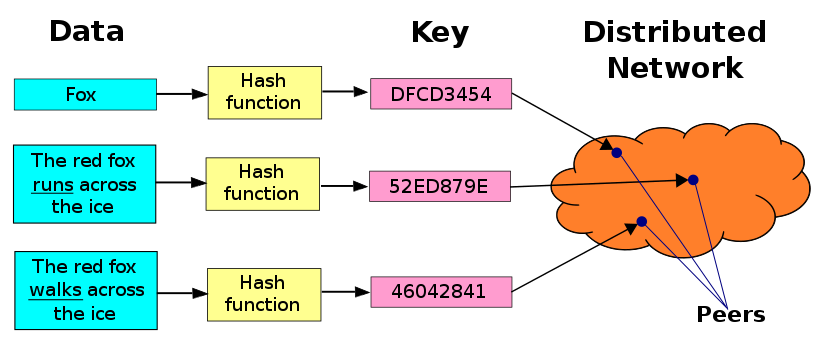
\includegraphics[width=0.6\textwidth]{figures/DHT}
  \caption[Distributed Hash Table] {
    Door het vertalen van data naar een cryptografische sleutel is het mogelijk om aan de hand van de sleutel de data op te vragen aan peers die de data bezitten.
  }
  \label{DHT}
\end{wrapfigure}

\textbf{Consensus}

Consensus is een dynamische manier van het behalen van overeenstemming in een groep. In blockchain implementaties wordt het gebruikt om overeenstemming te behalen over de staat van het netwerk en de volgorde waarin transacties gedaan zijn. Met het consensus algoritme wordt er een zekere mate van veiligheid gewaarborgd, waardoor het voor een kwaadwillende deelnemer (bijna) onmogelijk dient te zijn om het netwerk te beïnvloeden. Het kan voorkomen dat een kwaadwillende deelnemer probeert het netwerk te beïnvloeden waardoor er tegenstrijdige consensus kan optreden en een \gls{fork} ontstaat in het netwerk.

\textbf{Fork}

Een \gls{fork} is een splitsing in het netwerk die veroorzaakt is door een verandering in het protocol of door het toedoen van kwaadwillende deelnemer(s). Er zijn hiervoor twee categorieën \glspl{fork}, een \gls{hard_fork} en een \gls{soft_fork}.

\paragraph{Soft fork}

is een verandering in het netwerk die terugwaartse compatibiliteit heeft met eerdere versies van het protocol. Als voorbeeld kan er voor gekozen worden dat in plaats van blocks een limiet hebben van 1MB, de regel aangepast wordt zodat blocks een grootte van 500K moeten hebben. Als een \gls{soft_fork} verkeerd gaat is het nog steeds mogelijk dat er een \gls{hard_fork} optreed \citep[Soft Fork]{coindesk:forks}.

\paragraph{Hard fork}

is een protocol update waarbij een nieuwe regel geïntroduceerd wordt, waardoor het netwerk geen compatibiliteit heeft met oudere versies. Dit zorgt ervoor dat deelnemers in het netwerk die een oudere versie hebben, de nieuwe transacties als invalide beschouwen. Een voorbeeld van een regel waarbij een \gls{hard_fork} ontstaat is bijvoorbeeld het ophogen van de block grootte naar 2MB in plaats van 1MB \citep[Hard Fork]{coindesk:forks}. 

\newpage
\textbf{\Glspl{node}}

Alhoewel de structuur van een Blockchain dezelfde structuur afdwingt voor de \glspl{node} in het netwerk, kunnen zij een verschillende rol spelen. Alle \glspl{node} binnen het netwerk valideren, verspreiden en ontdekken en onderhouden connecties met andere \glspl{node} binnen het netwerk. In fig. \ref{blockchain_node_types} is te zien welke services een  \gls{full_node} in het Bitcoin netwerk aanbiedt. 

\begin{wrapfigure}{r}{0.4\textwidth}
  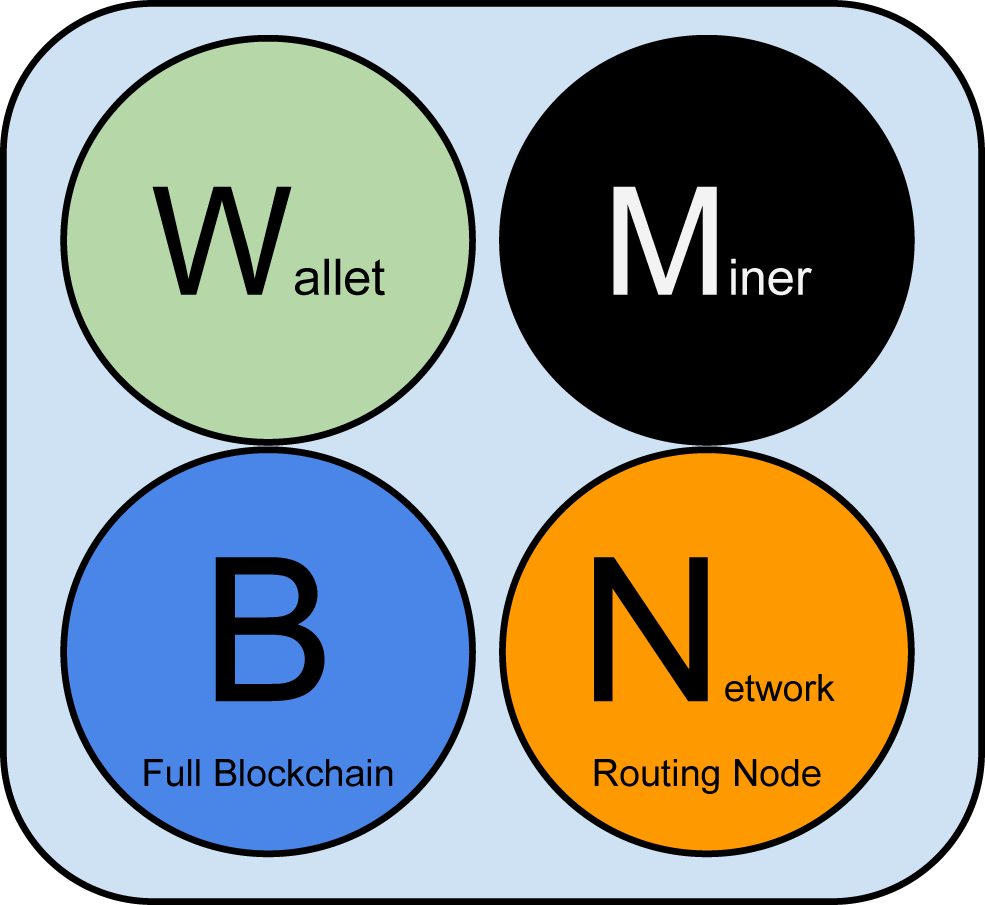
\includegraphics[width=0.4\textwidth]{figures/bitcoin_node_types}
  \caption[Bitcoin Node functionaliteiten] {
    Een bitcoin netwerk node die alle functies bevat: wallet, mining, blockchain database en netwerk routing, \citep[p.~172]{Antonopoulos:2014:MBU:2695500}.
  }
  \label{blockchain_node_types}
\end{wrapfigure}

Een \textbf{\gls{full_node}} is een collectie van functies, namelijk routing, de blockchain database, het mining proces en wallet services en bevat een gehele kopie van de actuele blockchain. Een \textbf{\gls{wallet_node}} is een deelnemer in het netwerk die een subset van de gehele blockchain bevat om transacties te versturen, verifiëren en ontvangen. De \textbf{\glspl{mining_node}} concurreren voor het creëren van een nieuw block door het uitvoeren van het Proof-of-Work algoritme. 

Alle \glspl{node} binnen het netwerk bieden gelijke diensten aan en kunnen gebruik maken van dezelfde diensten terwijl ze samenwerken door middel van een consensus protocol.

De verschillende services binnen het netwerk en de \gls{node} types die hieraan meewerken is dan ook een architecturale keuze over de indeling van het \acrshort{P2P} netwerk.


\newpage
\section{Identiteit}

\textit{
  In dit hoofdstuk wordt de vraag ``Waaruit bestaat het onderdeel Identity Management binnen Blockchain technologie?'' behandeld. Zoals beschreven in hoofdstuk \ref{chapter:blockchain} zijn anonimiteit en controleerbaarheid belangrijke eigenschappen van een Blockchain implementatie. Allereerst zal er beschreven worden wat identiteit inhoud binnen een Blockchain en welke mogelijke vormen van management er zijn. Het antwoord op deze vraag wordt gebruikt om zoektermen op te stellen en een afbakening te creëren voor de te onderzoeken protocollen.
}

In het vooronderzoek is er weinig gevonden over Identity Management en zelf wist ik dan ook niet goed wat dit onderdeel voor functionaliteiten bevat. In eerste instantie is er gekeken naar de verschillende types van Blockchain, waarbij gebruikers van het systeem autorisatie hebben tot bepaalde acties. Om een beter beeld te schetsen en de afbakening van het onderdeel compleet te maken voor het onderzoek is er besloten om een gesprek te houden met Pim Otte.

Uit dit gesprek is naar voren gekomen dat het Identity Management gedeelte gaat over hoe de Blockchain implementatie met public keys (de identiteit van een gebruiker) omgaat. Als tip werd er gegeven om te kijken naar de wallet software indien beschikbaar. Dit is software die de public- en private key beheert voor een gebruiker. Daarnaast is er ook een tip gegeven over het onderdeel Distributed Network. Om een goed beeld te krijgen van de aanvallen waar het netwerk tegen bestand is, is het handig om een threat model op te stellen.

Het onderdeel Identity Management beschrijft hoe de Blockchain omgaat met de identiteit van gebruiker die deel uitmaakt van het netwerk. Daarnaast is het mogelijk dat een bepaald type Blockchain meer doet dan alleen de identiteit van de gebruiker beheerd of maskeert. 

\subsection{Categorieën}

\cite{zheng2017overview} deelt Blockchain implementaties op in drie categorieën, waarin de zichtbaarheid en participatie in het consensus proces gelimiteerd.

\paragraph{Public} In een public Blockchain zijn alle transacties publiekelijk inzichtbaar en iedereen in het netwerk maakt onderdeel uit van het consensus proces. Dit wordt ook wel gezien als een permissionless Blockchain.

\paragraph{Consortium} In een consortium Blockchain is er een groep van vooraf geselecteerde nodes die deel uitmaken van het consensus proces. De consortium Blockchain wordt meestal gebruikt door meerdere organisaties en is gedeeltelijk gedecentraliseerd. Omdat bepaalde nodes geïdentificeerd dienen te worden wordt dit type Blockchain gezien als een permissioned Blockchain.

\clearpage
\paragraph{Private} In een private Blockchain worden alleen nodes van een specifieke organisatie toegelaten tot het consensus proces. Het wordt ook wel als een centraal netwerk gezien omdat het in volledige controle is van één organisatie. Omdat het hier gaat om volledige restrictie tot het Blockchain netwerk wordt dit type Blockchain gezien als een permissioned Blockchain.

In een consortium en een private Blockchain dient de gebruiker zich te identificeren aan de hand van een identiteit. Zoals eerder vermeld maakt Blockchain gebruik van een public- en private keys om de gebruiker te identificeren. Dit hanteert in zekere mate een permissie model waarbij de autorisatie van een gebruiker vastgelegd word aan de hand van de identificatie (i.e.\ de public key) die het netwerk gebruikt.

\subsection{Identificatie}

Identificatie wordt doorgaans gedaan aan de hand van een public key van een gebruiker. Een van de missies van Blockchain is totale anonimiteit, alleen zijn er een aantal problemen die volledige anonimiteit tegengaan. Om de terminologie duidelijk te maken wordt hieronder het verschil tussen pseudoniem en anoniem uitgelegd aan de hand van voorbeelden vanuit het Bitcoin protocol.

\begin{formal}
  ``Anonymity is the state of being not identifiable within a set of subjects, the anonymity set."
  \\ \cite{pfitzmann2001anonymity}.
\end{formal}

\paragraph{Pseudoniem} 

Bij een pseudoniem gaat er om een referentie naar de identiteit. 

\paragraph{Anoniem}







\newpage
\section{Obstakels}

In het vooronderzoek is er weinig gevonden over Identity Management en zelf wist ik dan ook niet goed wat dit onderdeel voor functionaliteiten bevat. In eerste instantie is er gekeken naar de verschillende types van Blockchain, waarbij gebruikers van het systeem autorisatie hebben tot bepaalde acties. Om een beter beeld te schetsen en de afbakening van het onderdeel compleet te maken voor het onderzoek is er besloten om een gesprek te houden met de Blockchain Expert.

Uit dit gesprek is naar voren gekomen dat het Identity Management gedeelte gaat over hoe de Blockchain implementatie met public keys (de identiteit van een gebruiker) omgaat. Als tip werd er gegeven om te kijken naar de wallet software indien beschikbaar. Dit is software die de public- en private key beheert voor een gebruiker. Daarnaast is er ook een tip gegeven over het onderdeel Distributed Network. Om een goed beeld te krijgen van de aanvallen waar het netwerk tegen bestand is, is het handig om een threat model op te stellen.
\section{Conclusie}

Naar aanleiding van de resultaten uit het vooronderzoek zijn er keuzes gemaakt die zich reflecteren in het onderzoek. Hieronder is per vraag beschreven over de implicaties die de resultaten gaven tegenover het onderzoek. 

Uit de vraag ``Waaruit bestaat het onderdeel Distributed Network binnen Blockchain technologie?'' is gebleken dat het consensus proces invloed heeft op de structuur van het netwerk. Het soort consensus zal dan ook gebruikt worden om de verschillende type Distributed Networks te onderscheiden. Ook zullen de verschillende type van nodes onderzocht worden om te identificeren welke bijdrage een bepaald type node levert om het netwerk in stand te houden. 

In de resultaten van de vraag ``Waaruit bestaat het onderdeel Identity Management binnen Blockchain technologie?'' is er geïdentificeerd dat er twee manieren zijn waarop de privacy van de gebruiker gewaarborgd wordt, namelijk of het een permissionless of permissioned Blockchain is en de identificatie van de gebruiker binnen het netwerk. Er wordt aangegeven dat het niveau van privacy en autorisatie ligt aan de categorie van waar de Blockchain deel van uitmaakt.

\begin{enumerate}[noitemsep]
  \item Zichtbaarheid van acties die de gebruiker onderneemt op de Blockchain.
  \item Autorisaties voor acties die de gebruiker wilt ondernemen op de Blockchain.
\end{enumerate}



  %next line adds the Bibliography to the contents page
  \addcontentsline{toc}{chapter}{Literatuurlijst}

  \bibliographystyle{apacite}  
  \setlength\bibsep{\baselineskip}  
  \bibliography{referenties}

  %now enable appendix numbering format and include any appendices
  \begin{appendices}
  \renewcommand\thesection{\Roman{section}}
  \renewcommand\thesubsection{\thesection.\roman{subsection}}

  \section{Opdrachtformulering}\label{appendix:opdrachtformulering}
  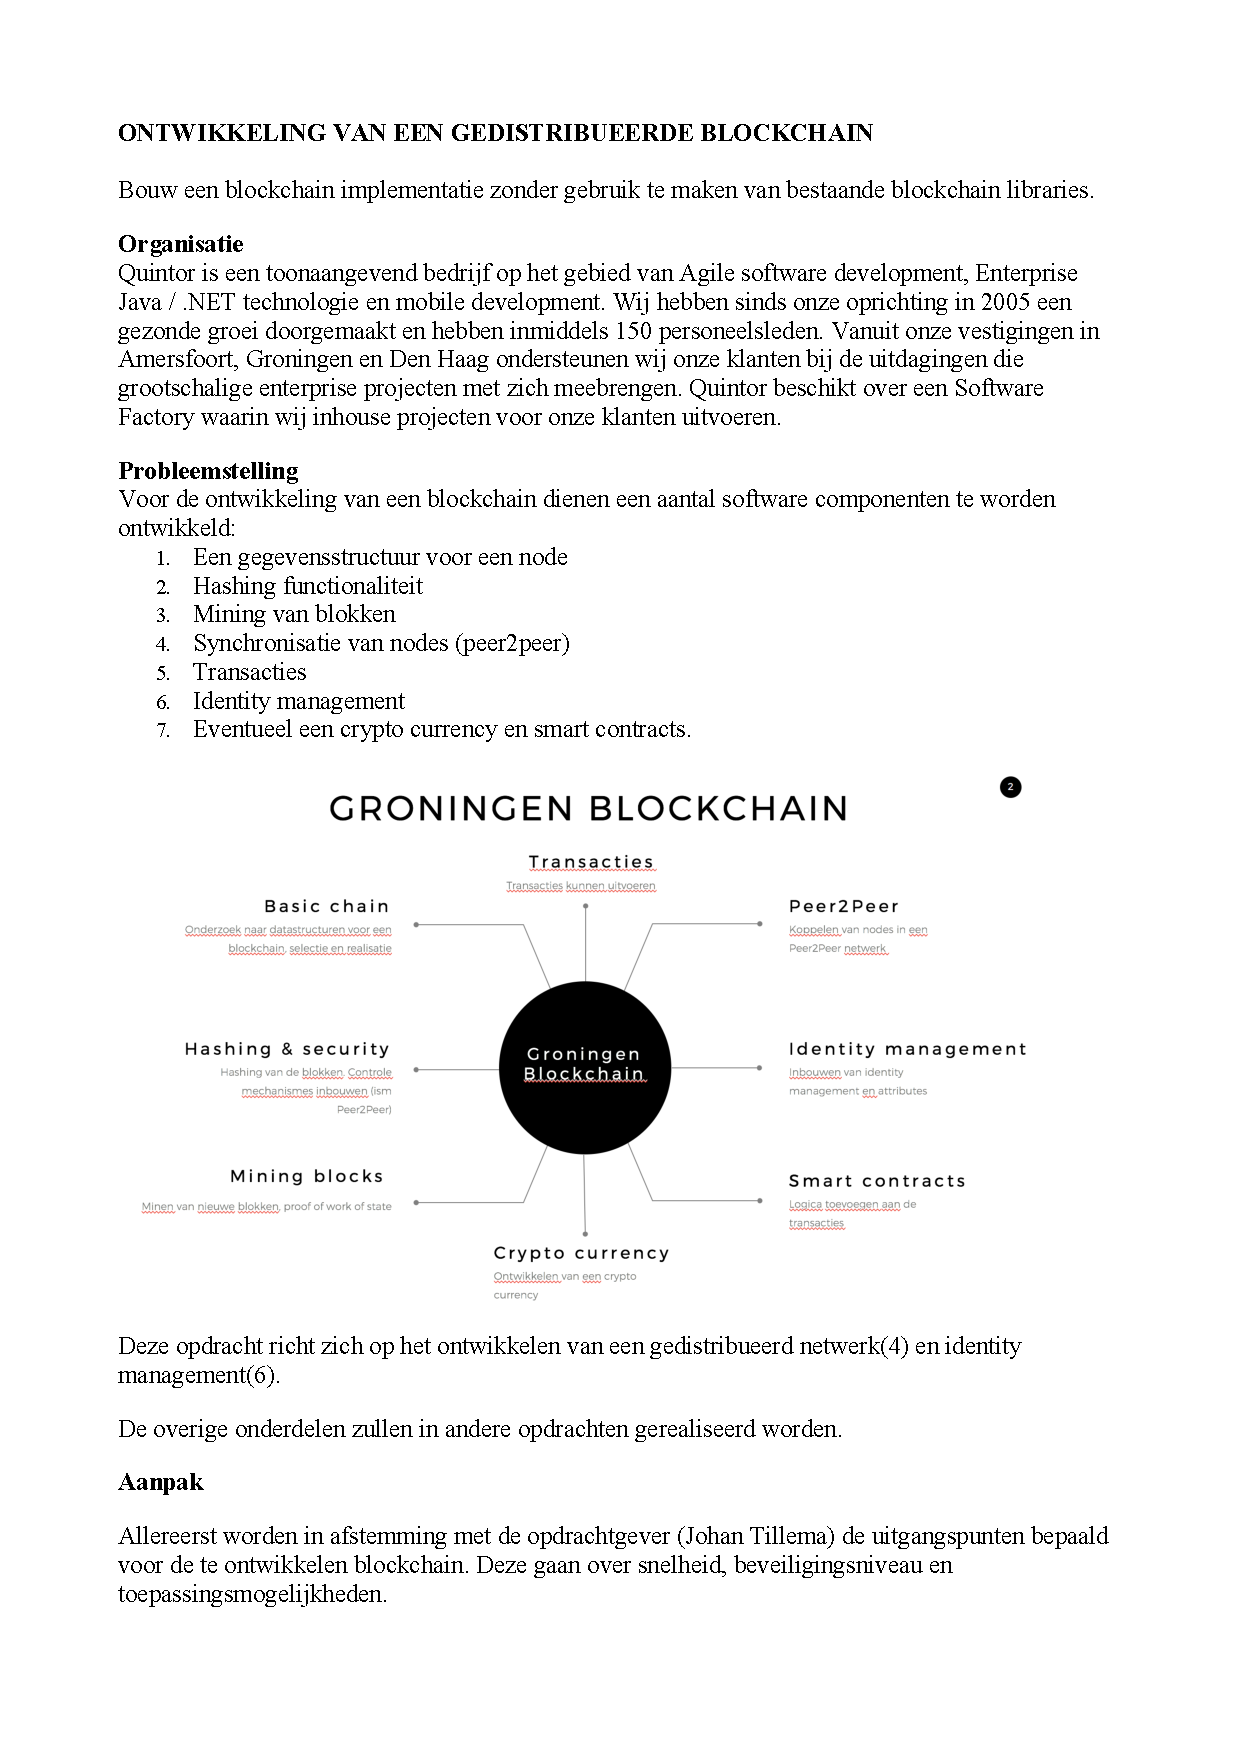
\includepdf[pages=-, frame=true, scale=0.7]{bijlages/quintor_opdracht.pdf}

  \section{Afstudeerplan}\label{appendix:afstudeerplan}
  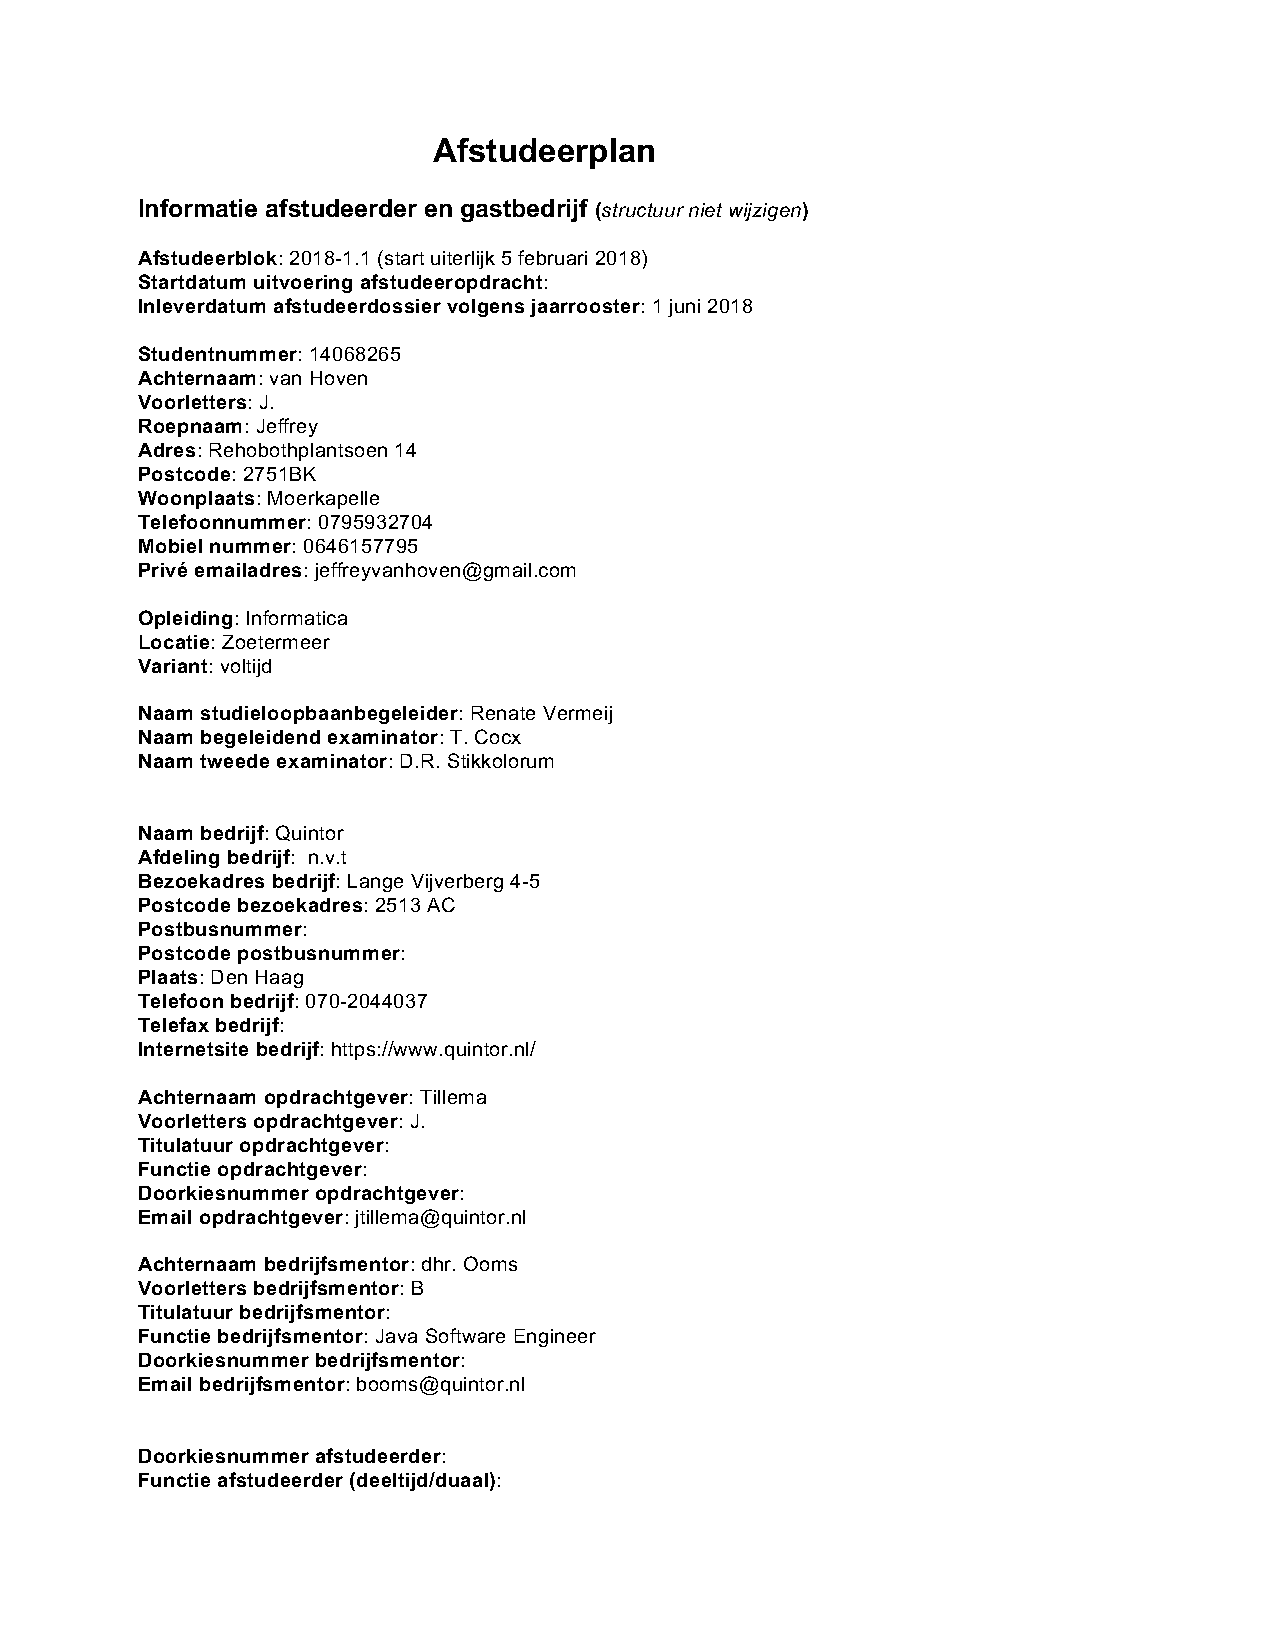
\includepdf[pages=-, frame=true, scale=0.7]{bijlages/afstudeerplan.pdf}

  \section{Plan van Aanpak}
  
\includepdf[pages=-, frame=true, scale=0.7]{bijlages/PvA/Aanpak.pdf}

  \section{Implementatie selectie}
  % Table generated by Excel2LaTeX from sheet 'Sheet2'
\begin{table}[htbp]
  \centering
  \caption{Bekeken implementaties uit de initiële selectie met de onderzochte attributen.}
  \begin{adjustbox}{width=25cm, height=6cm, angle=270}
    \begin{tabular}{llllrlp{17.915em}rlrrr}
      \toprule
      \textcolor[rgb]{ .188,  .329,  .588}{\textbf{Blockchain}} & \textcolor[rgb]{ .188,  .329,  .588}{\textbf{ Identity Management}} & \textcolor[rgb]{ .188,  .329,  .588}{\textbf{Whitepaper}} & \textcolor[rgb]{ .188,  .329,  .588}{\textbf{Open-source}} & \multicolumn{1}{l}{\textcolor[rgb]{ .188,  .329,  .588}{\textbf{In circulation since}}} & \textcolor[rgb]{ .188,  .329,  .588}{\textbf{Available Dapps development platform}} & \textcolor[rgb]{ .188,  .329,  .588}{\textbf{Notes}} & \multicolumn{1}{l}{\textcolor[rgb]{ .188,  .329,  .588}{\textbf{Consensus}}} & \textcolor[rgb]{ .188,  .329,  .588}{\textbf{Website}} & \multicolumn{1}{l}{\textcolor[rgb]{ .188,  .329,  .588}{\textbf{Repository}}} & \multicolumn{1}{l}{\textcolor[rgb]{ .188,  .329,  .588}{\textbf{Gebruikte talen}}} & \multicolumn{1}{l}{\textcolor[rgb]{ .188,  .329,  .588}{\textbf{Whitepaper url}}} \\
      \midrule
      \rowcolor[rgb]{ .267,  .447,  .769} \textcolor[rgb]{ 1,  1,  1}{\textbf{BitCoin}} & \cellcolor[rgb]{ 1,  .78,  .808}\textcolor[rgb]{ .612,  0,  .024}{No} & \cellcolor[rgb]{ .776,  .937,  .808}\textcolor[rgb]{ 0,  .38,  0}{Yes} & \cellcolor[rgb]{ .776,  .937,  .808}\textcolor[rgb]{ 0,  .38,  0}{Yes} & \cellcolor[rgb]{ .851,  .882,  .949}\textcolor[rgb]{ .188,  .329,  .588}{4/27/11} & \cellcolor[rgb]{ 1,  .78,  .808}\textcolor[rgb]{ .612,  0,  .024}{No} & \multicolumn{1}{r}{\cellcolor[rgb]{ .851,  .882,  .949}\textcolor[rgb]{ .188,  .329,  .588}{}} & \multicolumn{1}{l}{\cellcolor[rgb]{ .851,  .882,  .949}\textcolor[rgb]{ .188,  .329,  .588}{Proof of Work}} & \cellcolor[rgb]{ .851,  .882,  .949}\textcolor[rgb]{ .188,  .329,  .588}{https://bitcoin.org/nl/} & \multicolumn{1}{l}{\cellcolor[rgb]{ .851,  .882,  .949}\textcolor[rgb]{ .188,  .329,  .588}{https://github.com/bitcoin/}} & \multicolumn{1}{l}{\cellcolor[rgb]{ .851,  .882,  .949}\textcolor[rgb]{ .188,  .329,  .588}{C++}} & \multicolumn{1}{l}{\cellcolor[rgb]{ .851,  .882,  .949}\textcolor[rgb]{ .188,  .329,  .588}{https://bitcoin.org/bitcoin.pdf}} \\
      \rowcolor[rgb]{ .267,  .447,  .769} \textcolor[rgb]{ 1,  1,  1}{\textbf{Ethereum}} & \cellcolor[rgb]{ .776,  .937,  .808}\textcolor[rgb]{ 0,  .38,  0}{Yes} & \cellcolor[rgb]{ .776,  .937,  .808}\textcolor[rgb]{ 0,  .38,  0}{Yes} & \cellcolor[rgb]{ .776,  .937,  .808}\textcolor[rgb]{ 0,  .38,  0}{Yes} & \cellcolor[rgb]{ 1,  1,  1}\textcolor[rgb]{ .188,  .329,  .588}{7/30/15} & \cellcolor[rgb]{ .776,  .937,  .808}\textcolor[rgb]{ 0,  .38,  0}{Yes} & \multicolumn{1}{r}{\cellcolor[rgb]{ 1,  1,  1}\textcolor[rgb]{ .188,  .329,  .588}{}} & \multicolumn{1}{l}{\cellcolor[rgb]{ 1,  1,  1}\textcolor[rgb]{ .188,  .329,  .588}{Proof of Work}} & \cellcolor[rgb]{ 1,  1,  1}\textcolor[rgb]{ .188,  .329,  .588}{https://www.ethereum.org/} & \multicolumn{1}{l}{\cellcolor[rgb]{ 1,  1,  1}\textcolor[rgb]{ .188,  .329,  .588}{https://github.com/ethereum}} & \multicolumn{1}{l}{\cellcolor[rgb]{ 1,  1,  1}\textcolor[rgb]{ .188,  .329,  .588}{Go, C++}} & \multicolumn{1}{l}{\cellcolor[rgb]{ 1,  1,  1}\textcolor[rgb]{ .188,  .329,  .588}{https://github.com/ethereum/wiki/wiki/White-Paper}} \\
      \rowcolor[rgb]{ .267,  .447,  .769} \textcolor[rgb]{ 1,  1,  1}{\textbf{Tether}} & \cellcolor[rgb]{ 1,  .78,  .808}\textcolor[rgb]{ .612,  0,  .024}{No} & \cellcolor[rgb]{ .776,  .937,  .808}\textcolor[rgb]{ 0,  .38,  0}{Yes} & \cellcolor[rgb]{ 1,  .78,  .808}\textcolor[rgb]{ .612,  0,  .024}{No} & \cellcolor[rgb]{ .851,  .882,  .949}\textcolor[rgb]{ .188,  .329,  .588}{2015} & \cellcolor[rgb]{ .776,  .937,  .808}\textcolor[rgb]{ 0,  .38,  0}{Yes} & \cellcolor[rgb]{ .851,  .882,  .949}\textcolor[rgb]{ .188,  .329,  .588}{Fork from Bitcoin.} & \multicolumn{1}{l}{\cellcolor[rgb]{ .851,  .882,  .949}\textcolor[rgb]{ .188,  .329,  .588}{Proof of Reserves}} & \cellcolor[rgb]{ .851,  .882,  .949}\textcolor[rgb]{ .02,  .388,  .757}{https://www.tether.to/} & \multicolumn{1}{l}{\cellcolor[rgb]{ .851,  .882,  .949}\textcolor[rgb]{ .188,  .329,  .588}{https://bitbucket.org/tetherto/}} & \cellcolor[rgb]{ .851,  .882,  .949}\textcolor[rgb]{ .188,  .329,  .588}{} & \multicolumn{1}{l}{\cellcolor[rgb]{ .851,  .882,  .949}\textcolor[rgb]{ .188,  .329,  .588}{https://tether.to/wp-content/uploads/2016/06/TetherWhitePaper.pdf}} \\
      \rowcolor[rgb]{ .267,  .447,  .769} \textcolor[rgb]{ 1,  1,  1}{\textbf{Ripple}} & \cellcolor[rgb]{ 1,  .922,  .612}\textcolor[rgb]{ .612,  .341,  0}{Not sure} & \cellcolor[rgb]{ .776,  .937,  .808}\textcolor[rgb]{ 0,  .38,  0}{Yes} & \cellcolor[rgb]{ .776,  .937,  .808}\textcolor[rgb]{ 0,  .38,  0}{Yes} & \cellcolor[rgb]{ .851,  .882,  .949}\textcolor[rgb]{ .188,  .329,  .588}{2012} & \cellcolor[rgb]{ 1,  .78,  .808}\textcolor[rgb]{ .612,  0,  .024}{No} & \cellcolor[rgb]{ .851,  .882,  .949}\textcolor[rgb]{ .188,  .329,  .588}{Not really a Blockchain} & \multicolumn{1}{l}{\cellcolor[rgb]{ .851,  .882,  .949}\textcolor[rgb]{ .188,  .329,  .588}{Ripple Consensus Algorithm}} & \cellcolor[rgb]{ .851,  .882,  .949}\textcolor[rgb]{ .188,  .329,  .588}{https://ripple.com/} & \multicolumn{1}{l}{\cellcolor[rgb]{ .851,  .882,  .949}\textcolor[rgb]{ .188,  .329,  .588}{https://github.com/ripple}} & \multicolumn{1}{l}{\cellcolor[rgb]{ .851,  .882,  .949}\textcolor[rgb]{ .188,  .329,  .588}{C++}} & \multicolumn{1}{l}{\cellcolor[rgb]{ .851,  .882,  .949}\textcolor[rgb]{ .188,  .329,  .588}{https://ripple.com/files/ripple\_consensus\_whitepaper.pdf}} \\
      \rowcolor[rgb]{ .267,  .447,  .769} \textcolor[rgb]{ 1,  1,  1}{\textbf{EOS}} & \cellcolor[rgb]{ .776,  .937,  .808}\textcolor[rgb]{ 0,  .38,  0}{Yes} & \cellcolor[rgb]{ 1,  .922,  .612}\textcolor[rgb]{ .612,  .341,  0}{Sort of} & \cellcolor[rgb]{ .776,  .937,  .808}\textcolor[rgb]{ 0,  .38,  0}{Yes} & \cellcolor[rgb]{ 1,  1,  1}\textcolor[rgb]{ .188,  .329,  .588}{1/31/18} & \cellcolor[rgb]{ .776,  .937,  .808}\textcolor[rgb]{ 0,  .38,  0}{Yes} & \multicolumn{1}{r}{\cellcolor[rgb]{ 1,  1,  1}\textcolor[rgb]{ .188,  .329,  .588}{}} & \multicolumn{1}{l}{\cellcolor[rgb]{ 1,  1,  1}\textcolor[rgb]{ .188,  .329,  .588}{Delegated Proof of Stake}} & \cellcolor[rgb]{ 1,  1,  1}\textcolor[rgb]{ .188,  .329,  .588}{https://eos.io/} & \multicolumn{1}{l}{\cellcolor[rgb]{ 1,  1,  1}\textcolor[rgb]{ .188,  .329,  .588}{https://github.com/EOSIO}} & \multicolumn{1}{l}{\cellcolor[rgb]{ 1,  1,  1}\textcolor[rgb]{ .188,  .329,  .588}{C++}} & \cellcolor[rgb]{ 1,  1,  1}\textcolor[rgb]{ .188,  .329,  .588}{} \\
      \rowcolor[rgb]{ .267,  .447,  .769} \textcolor[rgb]{ 1,  1,  1}{\textbf{Cardano}} & \cellcolor[rgb]{ 1,  .922,  .612}\textcolor[rgb]{ .612,  .341,  0}{Not sure} & \cellcolor[rgb]{ .776,  .937,  .808}\textcolor[rgb]{ 0,  .38,  0}{Yes} & \cellcolor[rgb]{ 1,  .922,  .612}\textcolor[rgb]{ .612,  .341,  0}{Sort of} & \cellcolor[rgb]{ .851,  .882,  .949}\textcolor[rgb]{ .188,  .329,  .588}{11/29/17} & \cellcolor[rgb]{ .776,  .937,  .808}\textcolor[rgb]{ 0,  .38,  0}{Yes} & \cellcolor[rgb]{ .851,  .882,  .949}\textcolor[rgb]{ .188,  .329,  .588}{Only the "Settlement Layer" is open-source available} & \multicolumn{1}{l}{\cellcolor[rgb]{ .851,  .882,  .949}\textcolor[rgb]{ .188,  .329,  .588}{Proof of Stake}} & \cellcolor[rgb]{ .851,  .882,  .949}\textcolor[rgb]{ .188,  .329,  .588}{} & \multicolumn{1}{l}{\cellcolor[rgb]{ .851,  .882,  .949}\textcolor[rgb]{ .188,  .329,  .588}{https://github.com/input-output-hk/cardano-sl }} & \multicolumn{1}{l}{\cellcolor[rgb]{ .851,  .882,  .949}\textcolor[rgb]{ .188,  .329,  .588}{Haskell}} & \cellcolor[rgb]{ .851,  .882,  .949}\textcolor[rgb]{ .188,  .329,  .588}{} \\
      \rowcolor[rgb]{ .267,  .447,  .769} \textcolor[rgb]{ 1,  1,  1}{\textbf{NEO}} & \cellcolor[rgb]{ .776,  .937,  .808}\textcolor[rgb]{ 0,  .38,  0}{Yes} & \cellcolor[rgb]{ 1,  .78,  .808}\textcolor[rgb]{ .612,  0,  .024}{No} & \cellcolor[rgb]{ .776,  .937,  .808}\textcolor[rgb]{ 0,  .38,  0}{Yes} & \cellcolor[rgb]{ 1,  1,  1}\textcolor[rgb]{ .188,  .329,  .588}{2014} & \cellcolor[rgb]{ .776,  .937,  .808}\textcolor[rgb]{ 0,  .38,  0}{Yes} & \multicolumn{1}{r}{\cellcolor[rgb]{ 1,  1,  1}\textcolor[rgb]{ .188,  .329,  .588}{}} & \multicolumn{1}{l}{\cellcolor[rgb]{ 1,  1,  1}\textcolor[rgb]{ .188,  .329,  .588}{Delegated Byzantine Fault Tolerance}} & \cellcolor[rgb]{ 1,  1,  1}\textcolor[rgb]{ .188,  .329,  .588}{https://neo.org/} & \multicolumn{1}{l}{\cellcolor[rgb]{ 1,  1,  1}\textcolor[rgb]{ .188,  .329,  .588}{https://github.com/neo-project}} & \cellcolor[rgb]{ 1,  1,  1}\textcolor[rgb]{ .188,  .329,  .588}{} & \cellcolor[rgb]{ 1,  1,  1}\textcolor[rgb]{ .188,  .329,  .588}{} \\
      \rowcolor[rgb]{ .267,  .447,  .769} \textcolor[rgb]{ 1,  1,  1}{\textbf{Qtum}} & \cellcolor[rgb]{ .776,  .937,  .808}\textcolor[rgb]{ 0,  .38,  0}{Yes} & \cellcolor[rgb]{ .776,  .937,  .808}\textcolor[rgb]{ 0,  .38,  0}{Yes} & \cellcolor[rgb]{ 1,  .922,  .612}\textcolor[rgb]{ .612,  .341,  0}{Sort of} & \cellcolor[rgb]{ 1,  1,  1}11/13/17 & \cellcolor[rgb]{ .776,  .937,  .808}\textcolor[rgb]{ 0,  .38,  0}{Yes} & \cellcolor[rgb]{ .851,  .882,  .949}\textcolor[rgb]{ .188,  .329,  .588}{Adopts the UTXO model from Bitcoin while utilizing the Ethereum network. Implements PoS 3.0 as coined by the original Proof of Stake coin Blackcoin. Only the wallet is open-source.} & \multicolumn{1}{l}{\cellcolor[rgb]{ .851,  .882,  .949}\textcolor[rgb]{ .188,  .329,  .588}{Proof of Stake}} & \cellcolor[rgb]{ 1,  1,  1}https://qtum.org/en/ & \multicolumn{1}{l}{\cellcolor[rgb]{ 1,  1,  1}https://github.com/qtumproject} & \multicolumn{1}{l}{\cellcolor[rgb]{ .851,  .882,  .949}\textcolor[rgb]{ .188,  .329,  .588}{Wallet in C++}} & \multicolumn{1}{l}{\cellcolor[rgb]{ 1,  1,  1}https://qtum.org/uploads/files/a2772efe4dc8ed1100319c6480195fb1.pdf} \\
      \rowcolor[rgb]{ .267,  .447,  .769} \textcolor[rgb]{ 1,  1,  1}{\textbf{TRON}} & \cellcolor[rgb]{ 1,  .78,  .808}\textcolor[rgb]{ .612,  0,  .024}{No} & \cellcolor[rgb]{ .776,  .937,  .808}\textcolor[rgb]{ 0,  .38,  0}{Yes} & \cellcolor[rgb]{ 1,  .922,  .612}\textcolor[rgb]{ .612,  .341,  0}{Sort of} & \cellcolor[rgb]{ .851,  .882,  .949}\textcolor[rgb]{ .188,  .329,  .588}{2017} & \cellcolor[rgb]{ 1,  .78,  .808}\textcolor[rgb]{ .612,  0,  .024}{No} & \cellcolor[rgb]{ 1,  1,  1}\textcolor[rgb]{ .188,  .329,  .588}{Badly translated whitepaper and website.} & \multicolumn{1}{l}{\cellcolor[rgb]{ .851,  .882,  .949}\textcolor[rgb]{ .188,  .329,  .588}{Proof of Stake}} & \cellcolor[rgb]{ .851,  .882,  .949}\textcolor[rgb]{ .188,  .329,  .588}{https://tron.network/en.html} & \multicolumn{1}{l}{\cellcolor[rgb]{ .851,  .882,  .949}\textcolor[rgb]{ .188,  .329,  .588}{https://github.com/tronprotocol}} & \multicolumn{1}{l}{\cellcolor[rgb]{ .851,  .882,  .949}\textcolor[rgb]{ .188,  .329,  .588}{Java}} & \multicolumn{1}{l}{\cellcolor[rgb]{ .851,  .882,  .949}\textcolor[rgb]{ .188,  .329,  .588}{https://o836fhe91.qnssl.com/tron/whitebook/TronWhitepaper\_en.pdf}} \\
      \rowcolor[rgb]{ .267,  .447,  .769} \textcolor[rgb]{ 1,  1,  1}{\textbf{Status}} & \cellcolor[rgb]{ .776,  .937,  .808}\textcolor[rgb]{ 0,  .38,  0}{Yes} & \cellcolor[rgb]{ 1,  .78,  .808}\textcolor[rgb]{ .612,  0,  .024}{No} & \cellcolor[rgb]{ .776,  .937,  .808}\textcolor[rgb]{ 0,  .38,  0}{Yes} & \multicolumn{1}{l}{\cellcolor[rgb]{ 1,  1,  1}-} & \cellcolor[rgb]{ .776,  .937,  .808}\textcolor[rgb]{ 0,  .38,  0}{Yes} & \cellcolor[rgb]{ .851,  .882,  .949}\textcolor[rgb]{ .188,  .329,  .588}{Identity Management in form of usernames. Mobile client voor Ethereum, een Dapp die het mogelijk maakt om te interfacen met andere Dapps?} & \multicolumn{1}{l}{\cellcolor[rgb]{ .851,  .882,  .949}\textcolor[rgb]{ .188,  .329,  .588}{Proof of Work}} & \cellcolor[rgb]{ 1,  1,  1}https://status.im/ & \multicolumn{1}{l}{\cellcolor[rgb]{ 1,  1,  1}https://github.com/status-im} & \multicolumn{1}{l}{\cellcolor[rgb]{ .851,  .882,  .949}\textcolor[rgb]{ .188,  .329,  .588}{Go}} & \cellcolor[rgb]{ 1,  1,  1} \\
      \rowcolor[rgb]{ .267,  .447,  .769} \textcolor[rgb]{ 1,  1,  1}{\textbf{Stellar}} & \cellcolor[rgb]{ 1,  .922,  .612}\textcolor[rgb]{ .612,  .341,  0}{Not sure} & \cellcolor[rgb]{ 1,  .922,  .612}\textcolor[rgb]{ .612,  .341,  0}{Sort of} & \cellcolor[rgb]{ .776,  .937,  .808}\textcolor[rgb]{ 0,  .38,  0}{Yes} & \cellcolor[rgb]{ .851,  .882,  .949}\textcolor[rgb]{ .188,  .329,  .588}{2014} & \cellcolor[rgb]{ .776,  .937,  .808}\textcolor[rgb]{ 0,  .38,  0}{Yes} & \cellcolor[rgb]{ 1,  1,  1}\textcolor[rgb]{ .188,  .329,  .588}{Whitepaper only describes the consensus protocol, initially based on te Ripple protocol} & \multicolumn{1}{l}{\cellcolor[rgb]{ .851,  .882,  .949}\textcolor[rgb]{ .188,  .329,  .588}{Stellar Consensus Protocol}} & \cellcolor[rgb]{ .851,  .882,  .949}\textcolor[rgb]{ .188,  .329,  .588}{https://www.stellar.org} & \multicolumn{1}{l}{\cellcolor[rgb]{ .851,  .882,  .949}\textcolor[rgb]{ .188,  .329,  .588}{https://github.com/stellar}} & \multicolumn{1}{l}{\cellcolor[rgb]{ .851,  .882,  .949}\textcolor[rgb]{ .188,  .329,  .588}{C}} & \cellcolor[rgb]{ .851,  .882,  .949}\textcolor[rgb]{ .188,  .329,  .588}{} \\
      \rowcolor[rgb]{ .267,  .447,  .769} \textcolor[rgb]{ 1,  1,  1}{\textbf{Huobi Token}} & \cellcolor[rgb]{ 1,  .78,  .808}\textcolor[rgb]{ .612,  0,  .024}{No} & \cellcolor[rgb]{ 1,  .78,  .808}\textcolor[rgb]{ .612,  0,  .024}{No} & \cellcolor[rgb]{ 1,  .78,  .808}\textcolor[rgb]{ .612,  0,  .024}{No} & \cellcolor[rgb]{ 1,  1,  1} & \cellcolor[rgb]{ 1,  .78,  .808}\textcolor[rgb]{ .612,  0,  .024}{No} & \cellcolor[rgb]{ .851,  .882,  .949}\textcolor[rgb]{ .188,  .329,  .588}{Loyalty Blockchain, users cant buy but are awarded these tokens.} & \multicolumn{1}{l}{\cellcolor[rgb]{ .851,  .882,  .949}\textcolor[rgb]{ .188,  .329,  .588}{?}} & \cellcolor[rgb]{ 1,  1,  1}https://www.huobi.pro & \cellcolor[rgb]{ 1,  1,  1} & \cellcolor[rgb]{ 1,  1,  1} & \cellcolor[rgb]{ 1,  1,  1} \\
      \rowcolor[rgb]{ .267,  .447,  .769} \textcolor[rgb]{ 1,  1,  1}{\textbf{ATMCoin}} & \cellcolor[rgb]{ 1,  .922,  .612}\textcolor[rgb]{ .612,  .341,  0}{Not sure} & \cellcolor[rgb]{ 1,  .78,  .808}\textcolor[rgb]{ .612,  0,  .024}{No} & \cellcolor[rgb]{ 1,  .78,  .808}\textcolor[rgb]{ .612,  0,  .024}{No} & \multicolumn{1}{l}{\cellcolor[rgb]{ 1,  1,  1}-} & \cellcolor[rgb]{ 1,  .78,  .808}\textcolor[rgb]{ .612,  0,  .024}{No} & \cellcolor[rgb]{ 1,  1,  1}\textcolor[rgb]{ .188,  .329,  .588}{Doesnt look like anythings available for this crypto.} & \cellcolor[rgb]{ 1,  1,  1} & \cellcolor[rgb]{ 1,  1,  1}https://atmcoin.com/website/inicio & \cellcolor[rgb]{ 1,  1,  1} & \cellcolor[rgb]{ 1,  1,  1} & \multicolumn{1}{l}{\cellcolor[rgb]{ 1,  1,  1}https://atmcoin.com/contenidos/documentos/atmcoin\_whitepaper\_en-us.pdf} \\
      \rowcolor[rgb]{ .267,  .447,  .769} \textcolor[rgb]{ 1,  1,  1}{\textbf{Dash}} & \cellcolor[rgb]{ 1,  .78,  .808}\textcolor[rgb]{ .612,  0,  .024}{No} & \cellcolor[rgb]{ 1,  .922,  .612}\textcolor[rgb]{ .612,  .341,  0}{Sort of} & \cellcolor[rgb]{ .776,  .937,  .808}\textcolor[rgb]{ 0,  .38,  0}{Yes} & \cellcolor[rgb]{ .851,  .882,  .949}\textcolor[rgb]{ .188,  .329,  .588}{1/18/14} & \cellcolor[rgb]{ 1,  .922,  .612}\textcolor[rgb]{ .612,  .341,  0}{Not sure} & \cellcolor[rgb]{ .851,  .882,  .949}\textcolor[rgb]{ .188,  .329,  .588}{Initially named Xcoin (XCO), renamed to Darkcoin and then rebranded as Dash. Fork from LiteCoin. First self funded blockchain. Transaction fees go to a treasury, which funds development} & \multicolumn{1}{l}{\cellcolor[rgb]{ .851,  .882,  .949}\textcolor[rgb]{ .188,  .329,  .588}{Proof of Service}} & \cellcolor[rgb]{ .851,  .882,  .949}\textcolor[rgb]{ .188,  .329,  .588}{https://www.dash.org/} & \multicolumn{1}{l}{\cellcolor[rgb]{ .851,  .882,  .949}\textcolor[rgb]{ .188,  .329,  .588}{https://github.com/dashpay}} & \multicolumn{1}{l}{\cellcolor[rgb]{ .851,  .882,  .949}\textcolor[rgb]{ .188,  .329,  .588}{C++}} & \multicolumn{1}{l}{\cellcolor[rgb]{ .851,  .882,  .949}\textcolor[rgb]{ .188,  .329,  .588}{https://github.com/dashpay/dash/wiki/Whitepaper}} \\
      \rowcolor[rgb]{ .267,  .447,  .769} \textcolor[rgb]{ 1,  1,  1}{\textbf{VeChain}} & \cellcolor[rgb]{ 1,  .78,  .808}\textcolor[rgb]{ .612,  0,  .024}{No} & \cellcolor[rgb]{ 1,  .78,  .808}\textcolor[rgb]{ .612,  0,  .024}{No} & \cellcolor[rgb]{ 1,  .78,  .808}\textcolor[rgb]{ .612,  0,  .024}{No} & \cellcolor[rgb]{ 1,  1,  1}\textcolor[rgb]{ .188,  .329,  .588}{2015} & \cellcolor[rgb]{ 1,  .78,  .808}\textcolor[rgb]{ .612,  0,  .024}{No} & \cellcolor[rgb]{ 1,  1,  1}\textcolor[rgb]{ .188,  .329,  .588}{Chinese, private Blockchain for retail usage in combination with IoT.} & \cellcolor[rgb]{ 1,  1,  1}\textcolor[rgb]{ .188,  .329,  .588}{} & \cellcolor[rgb]{ 1,  1,  1}\textcolor[rgb]{ .188,  .329,  .588}{https://www.vechain.com/\#/} & \cellcolor[rgb]{ 1,  1,  1}\textcolor[rgb]{ .188,  .329,  .588}{} & \cellcolor[rgb]{ 1,  1,  1}\textcolor[rgb]{ .188,  .329,  .588}{} & \cellcolor[rgb]{ 1,  1,  1}\textcolor[rgb]{ .188,  .329,  .588}{} \\
      \rowcolor[rgb]{ .267,  .447,  .769} \textcolor[rgb]{ 1,  1,  1}{\textbf{Lisk}} & \cellcolor[rgb]{ .776,  .937,  .808}\textcolor[rgb]{ 0,  .38,  0}{Yes} & \cellcolor[rgb]{ 1,  .78,  .808}\textcolor[rgb]{ .612,  0,  .024}{No} & \cellcolor[rgb]{ .776,  .937,  .808}\textcolor[rgb]{ 0,  .38,  0}{Yes} & \cellcolor[rgb]{ 1,  1,  1}9/22/17 & \cellcolor[rgb]{ .776,  .937,  .808}\textcolor[rgb]{ 0,  .38,  0}{Yes} & \cellcolor[rgb]{ .851,  .882,  .949}\textcolor[rgb]{ .188,  .329,  .588}{Technical documentation available at https://lisk.io/documentation, albeit not in-depth.} & \multicolumn{1}{l}{\cellcolor[rgb]{ .851,  .882,  .949}\textcolor[rgb]{ .188,  .329,  .588}{Delegated Proof of Stake}} & \cellcolor[rgb]{ 1,  1,  1}https://lisk.io/ & \multicolumn{1}{l}{\cellcolor[rgb]{ 1,  1,  1}https://github.com/LiskHQ} & \multicolumn{1}{l}{\cellcolor[rgb]{ .851,  .882,  .949}\textcolor[rgb]{ .188,  .329,  .588}{JavaScript}} & \multicolumn{1}{l}{\cellcolor[rgb]{ 1,  1,  1}https://lisk.io/documentation/} \\
      \rowcolor[rgb]{ .267,  .447,  .769} \textcolor[rgb]{ 1,  1,  1}{\textbf{Monero}} & \cellcolor[rgb]{ .776,  .937,  .808}\textcolor[rgb]{ 0,  .38,  0}{Yes} & \cellcolor[rgb]{ .776,  .937,  .808}\textcolor[rgb]{ 0,  .38,  0}{Yes} & \cellcolor[rgb]{ .776,  .937,  .808}\textcolor[rgb]{ 0,  .38,  0}{Yes} & \cellcolor[rgb]{ .851,  .882,  .949}\textcolor[rgb]{ .188,  .329,  .588}{4/18/14} & \cellcolor[rgb]{ 1,  .78,  .808}\textcolor[rgb]{ .612,  0,  .024}{No} & \cellcolor[rgb]{ 1,  1,  1}\textcolor[rgb]{ .188,  .329,  .588}{Claims to be one and only fully anonimized Blockchain implementation} & \multicolumn{1}{l}{\cellcolor[rgb]{ .851,  .882,  .949}\textcolor[rgb]{ .188,  .329,  .588}{Proof of Work}} & \cellcolor[rgb]{ .851,  .882,  .949}\textcolor[rgb]{ .188,  .329,  .588}{https://getmonero.org/} & \multicolumn{1}{l}{\cellcolor[rgb]{ .851,  .882,  .949}\textcolor[rgb]{ .188,  .329,  .588}{https://github.com/monero-project}} & \multicolumn{1}{l}{\cellcolor[rgb]{ .851,  .882,  .949}\textcolor[rgb]{ .188,  .329,  .588}{C++}} & \multicolumn{1}{l}{\cellcolor[rgb]{ .851,  .882,  .949}\textcolor[rgb]{ .188,  .329,  .588}{https://downloads.getmonero.org/whitepaper\_annotated.pdf}} \\
      \rowcolor[rgb]{ .267,  .447,  .769} \textcolor[rgb]{ 1,  1,  1}{\textbf{Hshare}} & \cellcolor[rgb]{ .776,  .937,  .808}\textcolor[rgb]{ 0,  .38,  0}{Yes} & \cellcolor[rgb]{ .776,  .937,  .808}\textcolor[rgb]{ 0,  .38,  0}{Yes} & \cellcolor[rgb]{ .776,  .937,  .808}\textcolor[rgb]{ 0,  .38,  0}{Yes} & \cellcolor[rgb]{ 1,  1,  1} & \cellcolor[rgb]{ 1,  1,  1} & \cellcolor[rgb]{ .851,  .882,  .949}\textcolor[rgb]{ .188,  .329,  .588}{Uses black and white addresses} & \multicolumn{1}{l}{\cellcolor[rgb]{ .851,  .882,  .949}\textcolor[rgb]{ .188,  .329,  .588}{PoW + PoS}} & \cellcolor[rgb]{ 1,  1,  1}https://h.cash/ & \multicolumn{1}{l}{\cellcolor[rgb]{ 1,  1,  1}https://github.com/HcashOrg} & \multicolumn{1}{l}{\cellcolor[rgb]{ .851,  .882,  .949}\textcolor[rgb]{ .188,  .329,  .588}{C++}} & \cellcolor[rgb]{ 1,  1,  1} \\
      \rowcolor[rgb]{ .267,  .447,  .769} \textcolor[rgb]{ 1,  1,  1}{\textbf{ICON}} & \cellcolor[rgb]{ .776,  .937,  .808}\textcolor[rgb]{ 0,  .38,  0}{Yes} & \cellcolor[rgb]{ .776,  .937,  .808}\textcolor[rgb]{ 0,  .38,  0}{Yes} & \cellcolor[rgb]{ 1,  .78,  .808}\textcolor[rgb]{ .612,  0,  .024}{No} & \cellcolor[rgb]{ 1,  1,  1}\textcolor[rgb]{ .188,  .329,  .588}{} & \cellcolor[rgb]{ 1,  .922,  .612}\textcolor[rgb]{ .612,  .341,  0}{Not sure} & \multicolumn{1}{r}{\cellcolor[rgb]{ 1,  1,  1}\textcolor[rgb]{ .188,  .329,  .588}{}} & \multicolumn{1}{l}{\cellcolor[rgb]{ 1,  1,  1}\textcolor[rgb]{ .188,  .329,  .588}{Loop Fault Tolerance}} & \cellcolor[rgb]{ 1,  1,  1}\textcolor[rgb]{ .188,  .329,  .588}{https://icon.foundation/?lang=en} & \multicolumn{1}{l}{\cellcolor[rgb]{ 1,  1,  1}\textcolor[rgb]{ .188,  .329,  .588}{https://github.com/icon-foundation/}} & \cellcolor[rgb]{ 1,  1,  1}\textcolor[rgb]{ .188,  .329,  .588}{} & \multicolumn{1}{l}{\cellcolor[rgb]{ 1,  1,  1}\textcolor[rgb]{ .188,  .329,  .588}{https://icon.foundation/resources/whitepaper/ICON-Whitepaper-EN-Draft.pdf}} \\
      \rowcolor[rgb]{ .267,  .447,  .769} \textcolor[rgb]{ 1,  1,  1}{\textbf{Nano}} & \cellcolor[rgb]{ 1,  .78,  .808}\textcolor[rgb]{ .612,  0,  .024}{No} & \cellcolor[rgb]{ .776,  .937,  .808}\textcolor[rgb]{ 0,  .38,  0}{Yes} & \cellcolor[rgb]{ .776,  .937,  .808}\textcolor[rgb]{ 0,  .38,  0}{Yes} & \cellcolor[rgb]{ 1,  1,  1}\textcolor[rgb]{ .188,  .329,  .588}{} & \cellcolor[rgb]{ 1,  .78,  .808}\textcolor[rgb]{ .612,  0,  .024}{No} & \cellcolor[rgb]{ .851,  .882,  .949}\textcolor[rgb]{ .188,  .329,  .588}{Previously known as Raiblocks. Second blockchain that uses a tangle instead of a chain.} & \cellcolor[rgb]{ 1,  1,  1}\textcolor[rgb]{ .188,  .329,  .588}{} & \cellcolor[rgb]{ 1,  1,  1}\textcolor[rgb]{ .188,  .329,  .588}{https://nano.org/en} & \cellcolor[rgb]{ 1,  1,  1}\textcolor[rgb]{ .188,  .329,  .588}{} & \cellcolor[rgb]{ 1,  1,  1}\textcolor[rgb]{ .188,  .329,  .588}{} & \cellcolor[rgb]{ 1,  1,  1}\textcolor[rgb]{ .188,  .329,  .588}{} \\
      \cmidrule{2-6}\cmidrule{8-12}    
    \end{tabular}
  \end{adjustbox}
  \label{bijlage_selectie_implementatie}
\end{table}




  
  \section{Onderzoeksrapport}
  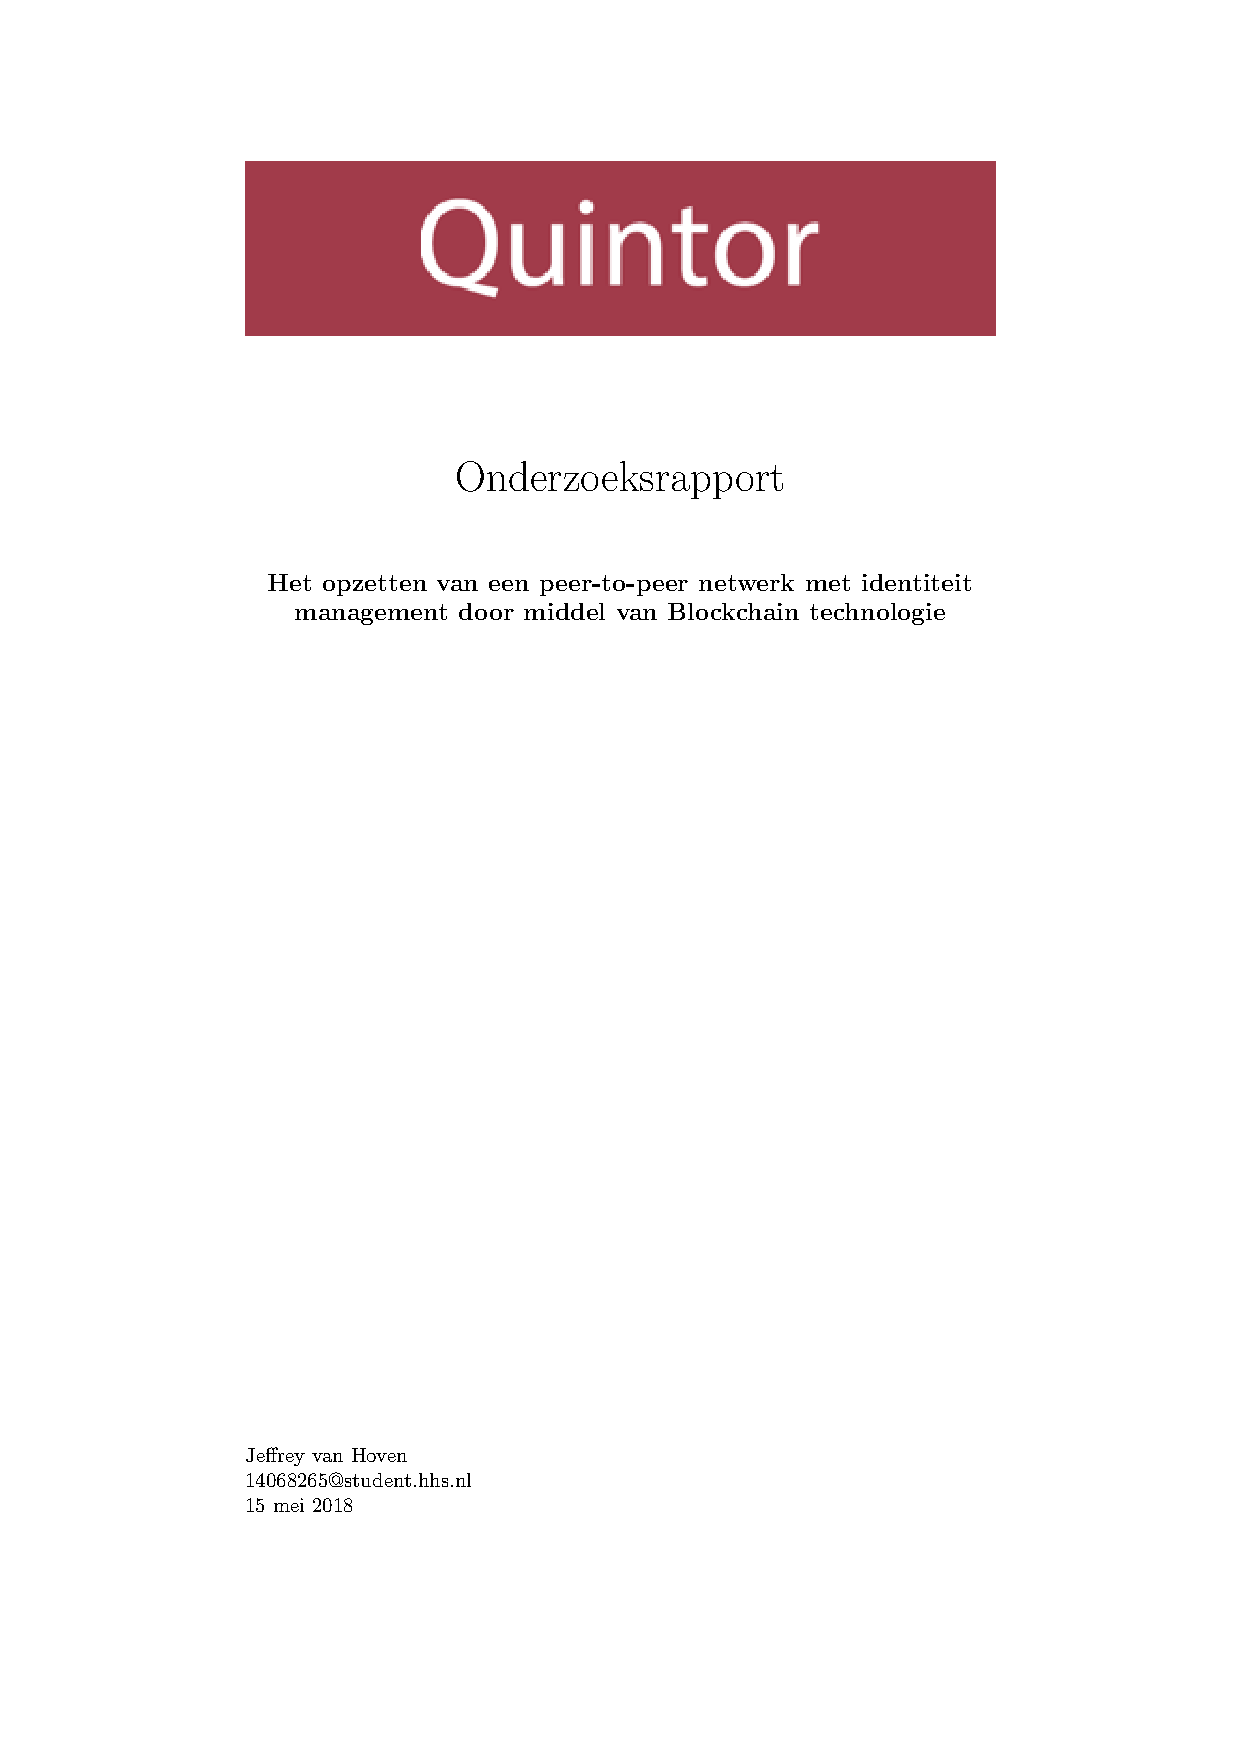
\includepdf[pages=-, frame=true, scale=0.7]{bijlages/Onderzoeksrapport/Onderzoeksrapport.pdf}

  \section{Adviesrapport}
  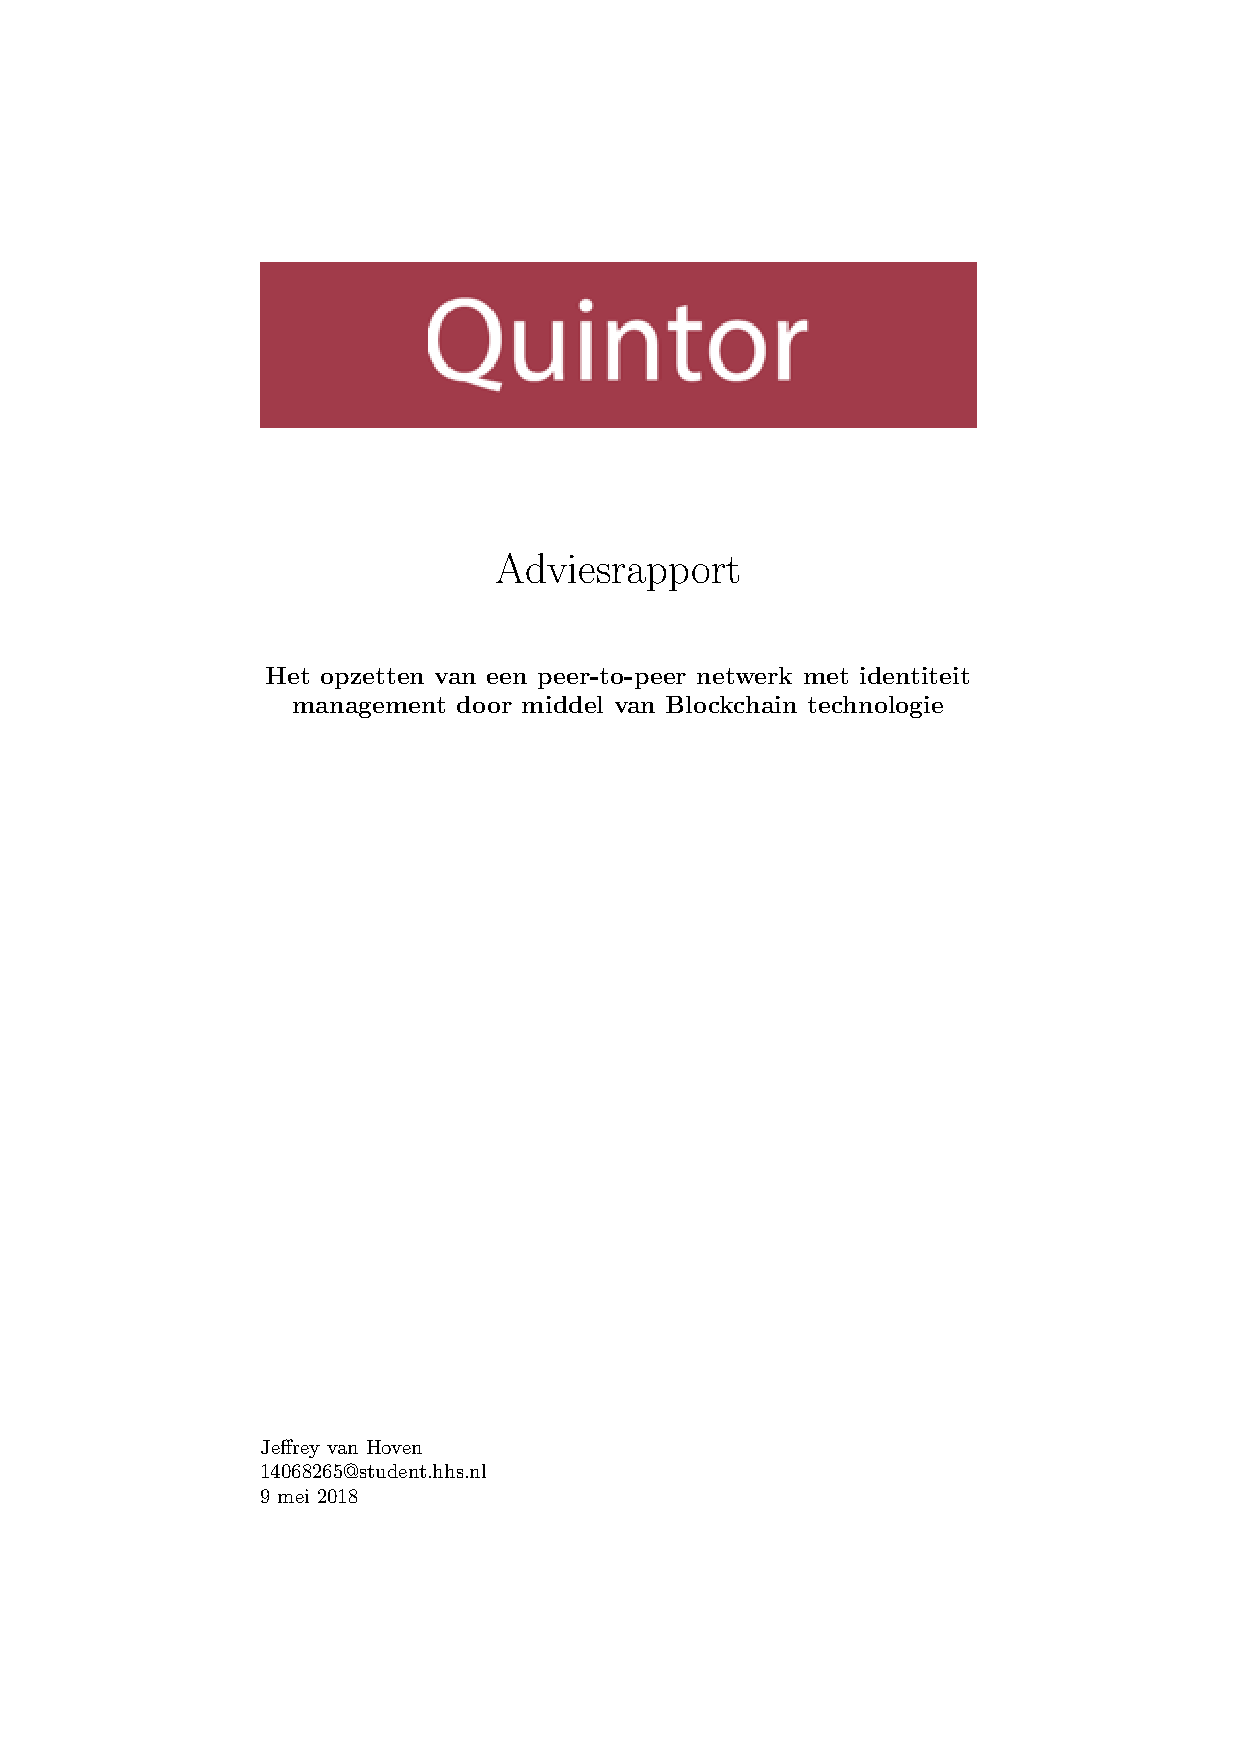
\includepdf[pages=-, frame=true, scale=0.7]{bijlages/Adviesrapport/Adviesrapport.pdf}

  \section{Voortgangsverslag}
  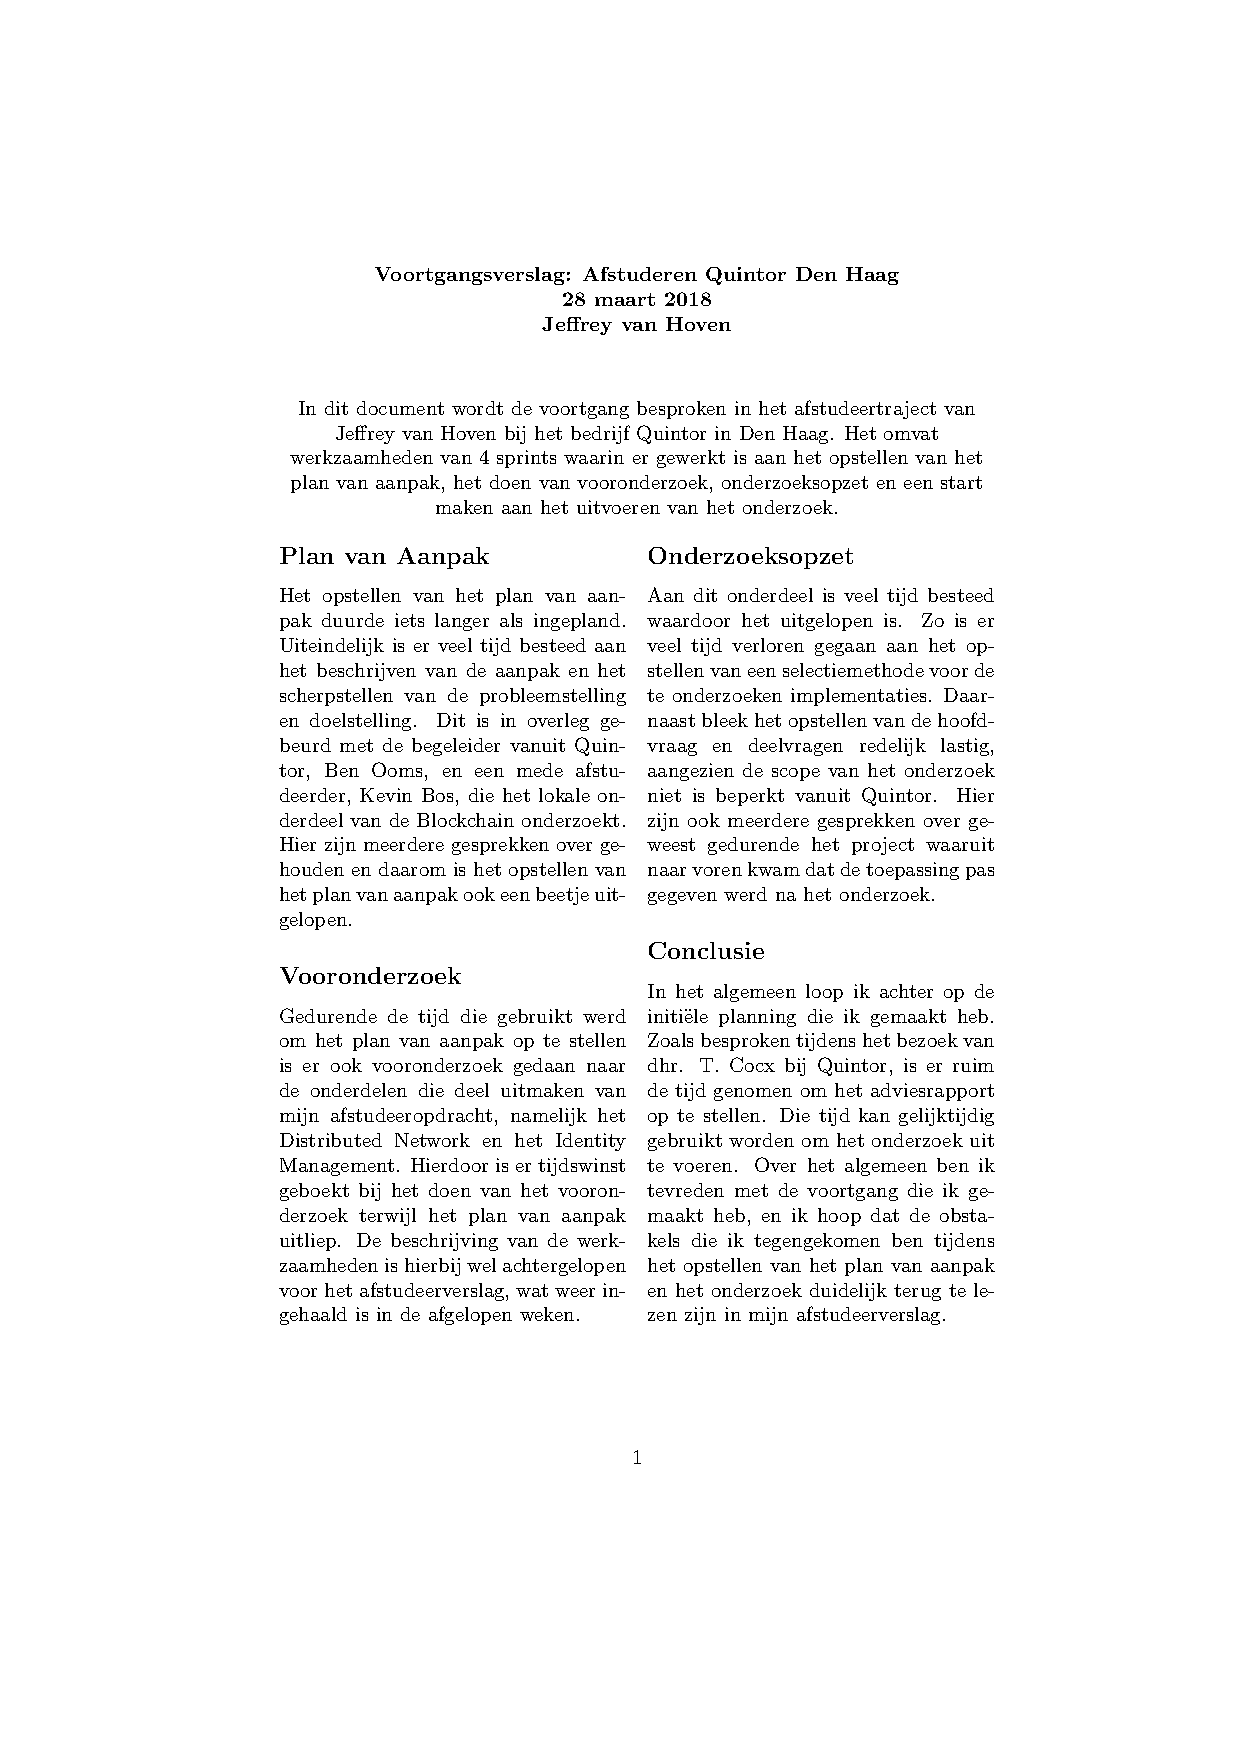
\includepdf[pages=-, frame=true, scale=0.7]{bijlages/Voortgangsverslag/Verslag.pdf}

  \section{Bezoekverslag}
  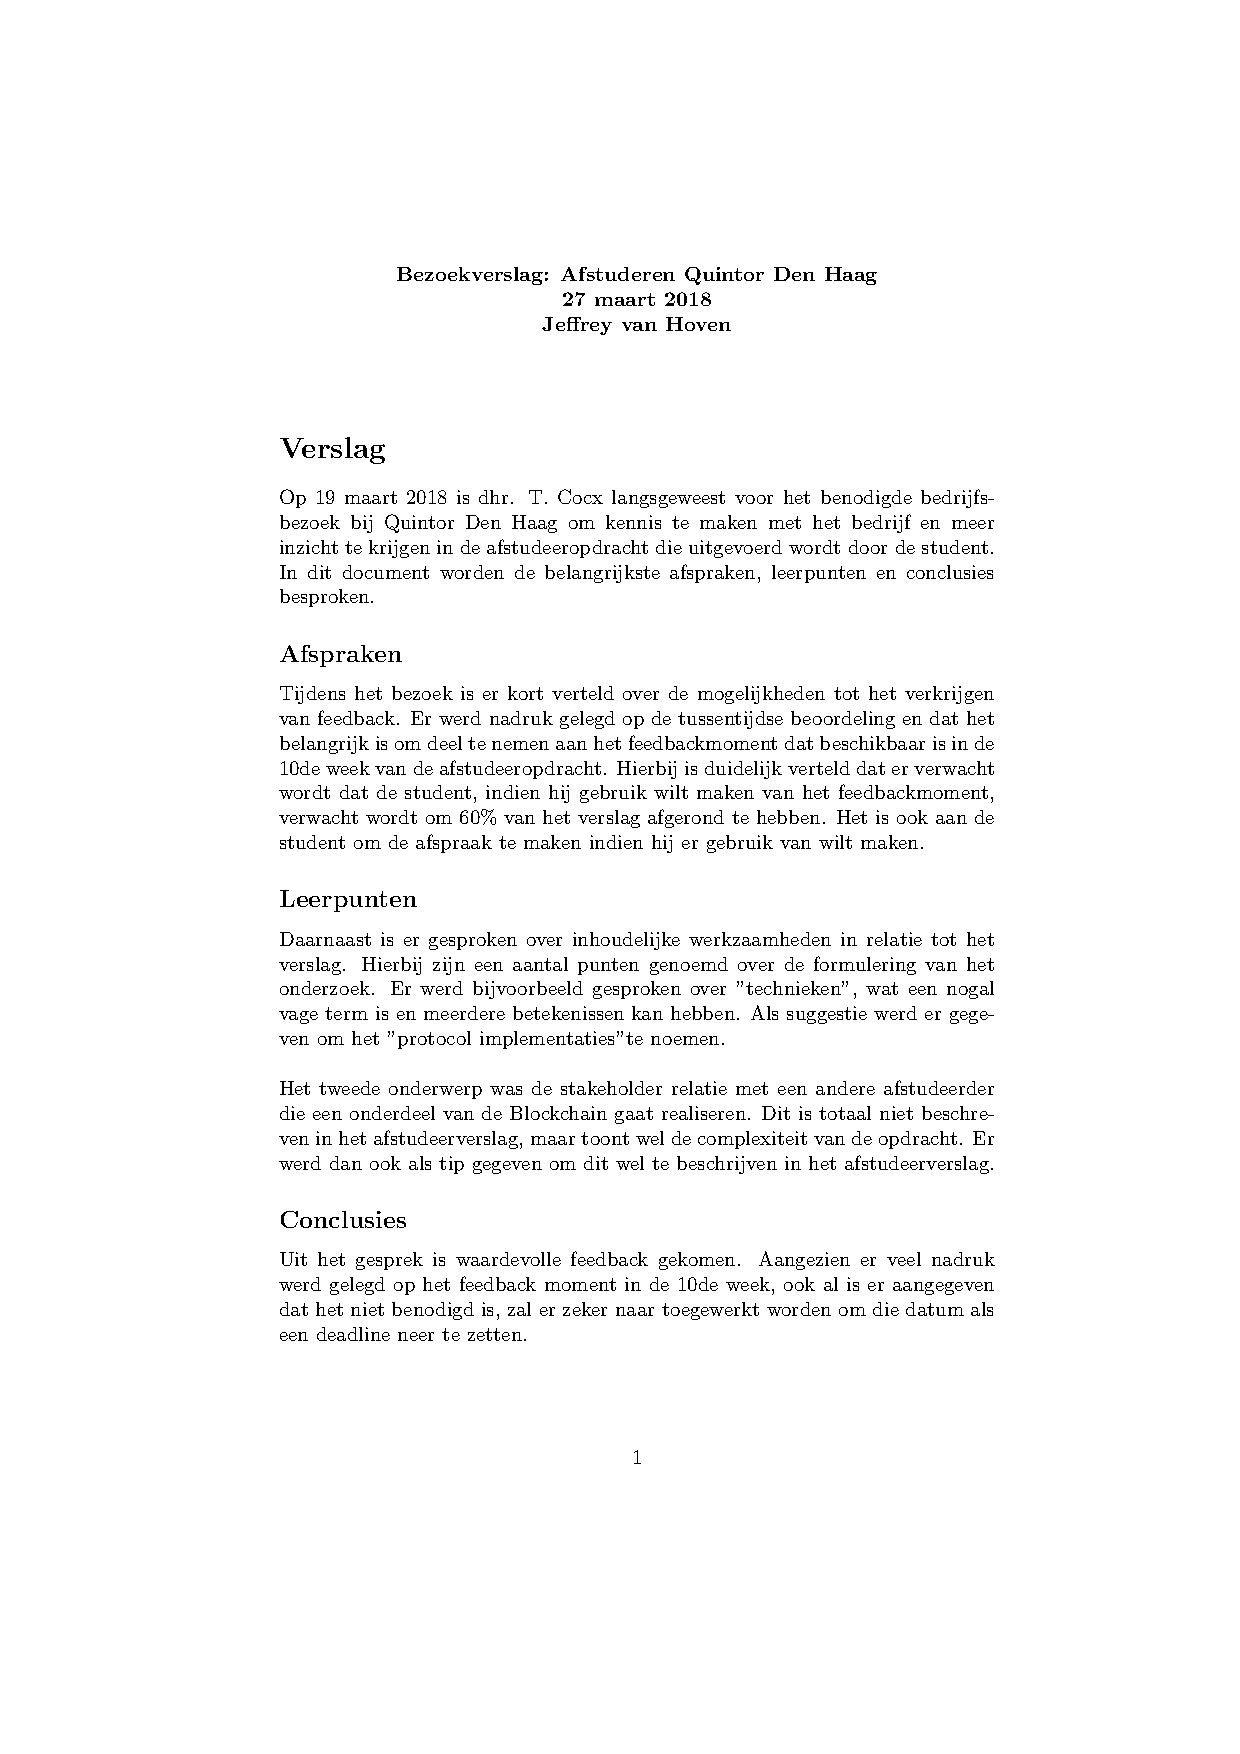
\includepdf[pages=-, frame=true, scale=0.7]{bijlages/Bezoek/Rapport.pdf}
  \addtocontents{toc}{\endgroup}
\end{appendices}
\end{document}
